\documentclass{document/thesisclass}
%% -------------------------
%% |    Thesis Settings    |
%% -------------------------
% english or ngerman (new german für neue deutsche Rechtschreibung statt german)
\SelectLanguage{english}
% details on this thesis
\newcommand{\thesisauthor}{Fabian Leven}
\newcommand{\thesistopic}{Analysis of Selected Models for Inelastic Electron-Scattering in the KATRIN Gaseous Tritium Source}
\newcommand{\thesisentopic}{}
\newcommand{\thesislongtopic}{}
\newcommand{\thesisinstitute}{Institute of Experimental Particle Physics (ETP)}
\newcommand{\thesisreviewerone}{Prof. Dr. G. Drexlin}
\newcommand{\thesisrevieweroneinstitute}{Institute of Experimental Particle Physics, KIT}
\newcommand{\thesisreviewertwo}{Dr. K. Valerius}
\newcommand{\thesisreviewertwoinstitute}{Institute for Nuclear Physics, KIT}
\newcommand{\thesisadvisorone}{M. Sc. M. Machatschek}
\newcommand{\thesisadvisoroneinstitute}{\thesisrevieweroneinstitute}

\newcommand{\thesisadvisortwo}{}
\newcommand{\thesistimestart}{July 15th, 2018} % on titlepage
\newcommand{\thesistimeend}{July 14th, 2019} % on titlepage
\newcommand{\thesistimehandin}{14.07.2019} % on second page 'preamble'
\newcommand{\thesispagehead}{\thesisentopic} % page heading
%% -----------------------
%% |    Abbreviations    |
%% -----------------------
\newcommand{\op}[1]{\operatorname{#1}}                 % to write operators that
                                                       % are not predefined;
                                                       % it's just an abbrev.
                                                       % for the long command

\newcommand{\arr}[2]{\begin{array}{#1}#2\end{array}}   % to create arrays. very 
                                                       % useful in math env

\renewcommand{\d}{\ensuremath{\mathop{}\!\mathrm{d}}}               % as the differential 
                                                       % operator, e.g. 
                                                       % \frac{\d x}{\d t}

\newcommand{\NN}{\mathbb{N}}                           % or change it to
\newcommand{\RR}{\mathbb{R}}                           % \mathbbm and include
\newcommand{\CC}{\mathbb{C}}                           % pkg bbm if you prefer

\newcommand{\pdb}[2]{\frac{\partial #1}{\partial #2}}  % partial derivative


%% -----------------------------------
%% |    Commands and Environments    |
%% -----------------------------------
\newcommand{\margtodo}                                 % used by \todo command
{\marginpar{\textbf{\textcolor{kitcolor}{ToDo}}}{}}
\newcommand{\todo}[1]
{{\textbf{\textcolor{kitcolor}{[\margtodo{}#1]}}}{}}   % for todo-notes inside 
                                                       % the document
\newenvironment{deprecated}                            % for something that you
{\begin{color}{gray}}{\end{color}}                     % want to use no more

\newcommand{\xcaption}[3]{\caption[#1]{\textbf{#2} #3}}% nice caption cmd for
                                                       % short and long descrip.

\newcommand{\xfigure}[5]{\begin{figure}[#1]            % a quick command for
\centering                                             % including graphics 
\includegraphics[scale=#2]{./fig/#3}                   % with all necessary vars
\xcaption{#4}{#5}
\label{fig:#3}
\end{figure}}

\newcommand{\xfigurerot}[5]{\begin{figure}[#1]        % same as above, only
\centering                                            % image is rotated
\includegraphics[angle=270,scale=#2]{./fig/#3}
\xcaption{#4}{#5}
\label{fig:#3}
\end{figure}}

\newcommand{\xtable}[4]{\begin{table}[#1]             % same for tables
\centering
\xcaption{#3}{#4}
\rowcolors{3}{gray!10}{white}
\include{./tab/#2}
\label{tab:#2}
\end{table}}

\newcommand{\kryptonEightyThree}{\ce{^{83m}Kr}}
%\newcommand{\eqref}[1]{\mbox(eq. \ref{eq:#1})}}
%% ------------------------------------
%% |    Quantum Mechanics and Math    |
%% ------------------------------------
\newcommand{\ket}[1]{\left|#1\right\rangle}           % \ket{X}  ->  |X>
\newcommand{\bra}[1]{\left\langle#1\right|}           % \bra{X}  ->  <X|
\newcommand{\braket}[2]                               % \braket{X}{Y}  ->  <X|Y>
{\left\langle#1 \middle| #2\right\rangle}
\newcommand{\bratenket}[3]                            % \bratenket{X}{Y}{Z}  ->
{\left\langle#1 \middle|\middle| #2 \middle|\middle|  % <X|Y|Z>
#3\right\rangle}
\newcommand{\anglemean}[1]                            % \anglemean{X}  ->  <X>
{\left\langle #1 \right\rangle}                       % \norm{X}  ->  || X ||
\newcommand{\norm}[1]{\left\lVert#1\right\rVert}

\newcommand{\updownarrows}                            % \ket\updownarrows  ->
{\text{\rotatebox[origin=c]{90}{$\rightleftarrows$}}} % |↑↓> (cmt is utf8!)
\newcommand{\downuparrows}                            % \ket\updownarrows  ->
{\text{\rotatebox[origin=c]{270}{$\rightleftarrows$}}}% |↓↑>
\newcommand{\neswarrows}                              % \ket\neswarrows  ->
{\text{\rotatebox[origin=c]{45}{$\rightleftarrows$}}} % |↗↙>
\newcommand{\swnearrows}                              % \ket\swnearrows  ->
{\text{\rotatebox[origin=c]{225}{$\rightleftarrows$}}}% |↙↗>

\newcommand{\cre}{c^\dagger}                          % annihalation operator
\newcommand{\anh}{c^{\vphantom{\dagger}}}             % creation operator
\newcommand{\numb}{n^{\vphantom{\dagger}}}            % number operator

\newcommand{\fullstop}{\text{\,.}}                    % fullstop or comma in
\newcommand{\comma}{\text{\,,}}                       % math mode for use
                                                      % after equations
                                                      
\newcommand{\vect}[1]{\boldsymbol{\mathbf{#1}}}      % bold face
\newcommand{\unitvect}[1]{\hat{\vect{#1}}}          % bold face with hat

\newcommand{\ii}{\mathrm{i}}

\DeclarePairedDelimiter\abs{\lvert}{\rvert}

\newcommand{\Conv}{%
  \mathop{\scalebox{1.5}{\raisebox{-0.2ex}{$\otimes$}}
  }
}

\newcommand{\conv}{\ensuremath{\otimes}}

\newcommand{\transp}[1]{{#1}^{\mathsf{T}}}
\newcommand{\euler}{\mathrm{e}}
\newcommand{\mean}[1]{\left\langle{#1}\right\rangle}
\pdfsuppresswarningpagegroup=1
\newcommandx{\inputpdftex}[2][1=\linewidth]{	    
    \begin{center}
        \def\svgwidth{#1}
        \graphicspath{{#2/}}
        \input{#2/img.pdf_tex}
    \end{center}
}
\newcommand{\neutrino}{\upnu}
\newcommand{\eneutrino}{\neutrino_\mathrm{e}}
\newcommand{\muneutrino}{\neutrino_\upmu}
\newcommand{\taueutrino}{\neutrino_\uptau}


\newcommand{\aeneutrino}{\bar{\upnu}_{\mathrm{e}}}
\newcommand\brabar{\scalebox{.4}{(}\raisebox{-1.5pt}{--}\scalebox{.4}{)}} 
\newcommand{\maybeaneutrino}{\stackrel{\brabar}{\upnu}}
\input{include/commands/my-abbreviations.tex}




%% ---------------------
%% |    PDF - Setup    |
%% ---------------------
% This information will appear embed into the PDF file as meta data, but will 
% not be printed anywhere
\hypersetup
{
    pdfauthor={\thesisauthor},
    pdftitle={\thesistopic},
    pdfsubject={\thesistopic},
    pdfkeywords={kit,physik,\thesisauthor}
}
%% --------------------------------------
%% |    Settings for Word Separation    |
%% --------------------------------------
% Help for separation:
% In German package the following hints are additionally available:
% "- = Additional separation
% "| = Suppress ligation and possible separation (e.g. Schaf"|fell)
% "~ = Hyphenation without separation (e.g. bergauf und "~ab)
% "= = Hyphenation with separation before and after
% "" = Separation without a hyphenation (e.g. und/""oder)

% Describe separation hints here:
\hyphenation
{
    über-nom-me-nen an-ge-ge-be-nen
    %Pro-to-koll-in-stan-zen
    %Ma-na-ge-ment  Netz-werk-ele-men-ten
    %Netz-werk Netz-werk-re-ser-vie-rung
    %Netz-werk-adap-ter Fein-ju-stier-ung
    %Da-ten-strom-spe-zi-fi-ka-tion Pa-ket-rumpf
    %Kon-troll-in-stanz
}

\begin{document}
    \FrontMatter

    % coordinates for background border
\newcommand{\diameter}{20}
\newcommand{\xone}{-15}
\newcommand{\xtwo}{160}
\newcommand{\yone}{15}
\newcommand{\ytwo}{-253}




\begin{titlepage}
    % background border
    \begin{tikzpicture}[overlay]
    \draw[color=gray]
            (\xone mm, \yone mm)
      -- (\xtwo mm, \yone mm)
    arc (90:0:\diameter pt)
      -- (\xtwo mm + \diameter pt , \ytwo mm)
        -- (\xone mm + \diameter pt , \ytwo mm)
    arc (270:180:\diameter pt)
        -- (\xone mm, \yone mm);
    \end{tikzpicture}



    % KIT image and sign for faculty of physics
    \begin{textblock}{10}[0,0](4.5,2.5)
        
\includegraphics[width=.25\textwidth]{document/kitlogo.pdf}
    \end{textblock}
    \changefont{phv}{m}{n}    % helvetica
    %\begin{textblock}{10}[0,0](5.5,2.2)
    %    \begin{flushright}
    %        \Large FAKULTÄT FÜR PHYSIK\\\thesisinstitute
    %    \end{flushright}
    %\end{textblock}



    % horizontal line
    %\begin{textblock}{10}[0,0](4.2,3.1)
    %    \begin{tikzpicture}[overlay]
    %    \draw[color=gray]
    %            (\xone mm + 5 mm, -12 mm)
    %      -- (\xtwo mm + \diameter pt - 5 mm, -12 mm);
    %    \end{tikzpicture}
    %\end{textblock}



    % begin of text part
    \changefont{phv}{m}{n}    % helvetica
    \centering



    % thesis topic (en and ge)
    \vspace*{3cm}
    \Huge\thesistopic\\
    %\huge(\thesisentopic)\\



    % author name and institute
    \vspace*{2cm}
    \Large Master's thesis of\\
    \vspace*{1cm} 
    \huge\thesisauthor\\
    \vspace*{1cm}
    \Large at the \thesisinstitute \\ of the Department of Physics \\ at the Karlsruhe Institute of Technology



    % possible frontimage - thanks to JabberWok
    % for publishing the img under GNU Document License
    \vspace*{1.5cm}



    % examiners (Referenten)
    \vspace*{1.5cm}
    \Large
    \begin{center}
        \begin{tabular}[ht]{l c l}
        \iflanguage{english}{Reviewer}{Referent}: 
            & \hfill & \thesisreviewerone\\
            & \hfill & \thesisrevieweroneinstitute\\
        \iflanguage{english}{Second Reviewer}{Korreferent}: 
            & \hfill & \thesisreviewertwo\\
            & \hfill & \thesisreviewertwoinstitute\\
        % uncomment if you want to provide info on your advisors
        \iflanguage{english}{Advisor}{Betreuender Mitarbeiter}: 
            & \hfill & \thesisadvisorone\\
            & \hfill & \thesisadvisoroneinstitute\\
        %\iflanguage{english}{Second Advisor}{Zweiter betreuender Mitarbeiter}: 
        %    & \hfill & \thesisadvisortwo\\
        \end{tabular}
    \end{center}



    % working time
    \vspace{1cm}
    \begin{center}
        \large{ \thesistimestart \hspace*{0.25cm} -- %
                                   \hspace*{0.25cm} \thesistimeend}
    \end{center}



    % lowest text blocks concerning the KIT
    \begin{textblock}{10}[0,0](0.35,16.8)
        \tiny{KIT – Die Forschungsuniversität in der Helmholtz-Gemeinschaft}
    \end{textblock}
    \begin{textblock}{10}[0,0](11,16.75)
        \large{\textbf{www.kit.edu}}
    \end{textblock}
\end{titlepage}

    \chapter*{Erklärung der Selbstständigkeit}
Ich versichere, dass ich diese Arbeit selbstständig verfasst habe und keine %
anderen als die angegebenen Quellen und Hilfsmittel benutzt habe, die %
wörtlich oder inhaltlich übernommenen Stellen als solche kenntlich gemacht und %
die Satzung des KIT zur Sicherung guter wissenschaftlicher Praxis in der %
gültigen Fassung vom 24.05.2018 beachtet habe.\\

\vspace{1cm}

\renewcommand{\arraystretch}{0} % for spacing in the tabular environment

\begin{flushright}
	\begin{tabular}{rr}
		Karlsruhe, den \thesistimehandin, & \hspace*{5cm}\\[0mm]
		\cline{2-2}\\[2mm]    % the last line has height 2mm due
		& \thesisauthor       % to \arraystretch=0
	\end{tabular}
\end{flushright}

\vfill

\begin{flushright}
	Als Prüfungsexemplar genehmigt von\\
	\vspace{1cm}
	\begin{tabular}{rr}
		Karlsruhe, den \thesistimehandin, & \hspace*{5cm}\\[0mm]
		\cline{2-2}\\[2mm]    % the last line has height 2mm due
		& \thesisreviewerone  % to \arraystretch=0
	\end{tabular}
\end{flushright}

\renewcommand{\arraystretch}{1}

\cleardoublepage


    \begingroup \let\clearpage\relax    % in order to avoid listoffigures and
    \tableofcontents                    % listoftables on new pages
    \listoffigures
    \listoftables
    \endgroup
    \cleardoublepage

    \MainMatter
    
    \newacronym{standardmodel}{SM}{Standard Model of particle physics}
\newacronym{lep}{LEP}{Large Electron Positron Collider}
\chapter{Neutrino Physics}
    
    \section{Neutrinos until the 1960s}
    The rich history of neutrino physics covers more than a century. The following paragraphs outline selected milestones on the way to their today's understanding.
    
    In 1895 Becquerel reported results on experiments with phosphorescent substances, especially uranium salts, on photographic plates \cite{Becquerel:1}. His experiments are marked as the discovery of radioactivity and triggered manifold subsequent investigations.
    
    In 1899 Rutherford published a classification of radioactive decays into $\upalpha$ and $\upbeta$ types according to their penetration strength \cite{Rutherford:1}.
    
    In 1900 Becquerel determined the mass-charge-ratio of $\upbeta$ decay particles and identified them as the electron previously described by Thomson \cite{Becquerel:2} \cite{Thomson:1}.
    
    In 1914 Chadwick measured a continuous electron energy spectrum in the $\upbeta$ decay ($\upbeta$ spectrum) of lead-214 and bismuth-214 \cite{Chadwick:1}.
    
    In 1927 Ellis and Wooster conducted a calorimetric measurement of the $\upbeta$ decay energy of radium and demonstrated that the continuity of the $\upbeta$ spectrum was intrinsic to the decay as opposed to caused by secondary effects as e.g. scattering of the electrons within an atom \cite{Ellis:1}.
    
    In 1930 a $\upbeta$ decay was thought of as a two-body-decay $A \rightarrow B + C$. Assuming relativistic kinematics, especially conservation of energy and momentum, in a two-body-decay the momenta of the daughter particles $B$ and $C$ are solely determined by their masses and the energy constitution of the parent particle $A$. According to Bohr there was no reason to believe that different nuclei of the same element $A$ should have a different energy constitution in a $\upbeta$ decay. Hence, the continuity of the $\upbeta$ spectrum could not be explained \cite{Bohr:1}. As a possible solution Pauli suggested the $\upbeta$ decay to be a three-body-decay and postulated a electrically neutral particle that carries part of the decay energy \cite{Pauli1930}.
    
    In 1934 Fermi developed a quantitative theory of $\upbeta$ decay that could describe the preceding experimental results. It comprises a four-fermion contact interaction respectively a three-body-decay model. It was the first description of the so-called ``weak interaction''. Furthermore, Fermi coined the term ``neutrino'' for the particle postulated by Pauli. \cite{Fermi1934}
    
    Fermi's theory inspired the idea to use the so-called ``inverse $\upbeta$ decay'' or ``neutrino capture'' to detect neutrinos, which in today's nomenclature is written as
    \begin{equation*}
        \aeneutrino + \proton \rightarrow \neutron + \positron \fullstop
    \end{equation*}
    In 1956 Cowan anrd Reines published results of a corresponding experiment. It was conducted using the sufficiently high neutrino flux of the nuclear reactor of the Savannah River Plant. The neutrinos originating in the reactor passed a tank of water and cadmium chloride triggering the above process. The emerging neutron was captured by the cadmium which emitted a photon in a \SIrange{3}{11}{MeV} range. The emerging positron annihilated with an electron which produced two photons of \SI{0.5}{MeV} each. A coincidence measurement of the corresponding photons enabled discriminating signal and background events. Based on their results they reported the free neutrino's discovery. \cite{Cowan103}
    
    In the same year, 1956, Lee and Yang published an article on parity conservation. Parity conservation implies that a mirrored physical process behaves the same as its non-mirrored counterpart. They pointed out that parity conservation might be violated in weak interactions and suggested several probing methods. \cite{Lee1956}
    
    In 1957 Wu et. al. conducted one of the corresponding probing methods based on $\upbeta$ decay. The parity operation respectively ``the mirroring'' corresponded a change of the magnetic field orientation in the experiment. The results showed that parity is violated. \cite{Wu1957}
    
    In 1958 Goldhaber et al. measured the helicity $H$ of the neutrino. Its helicity is defined as $ H = \unitvect{\sigma} \cdot \unitvect{p}$, where $\unitvect{\sigma}$ is the spin unit vector and $\unitvect{p}$ is the momentum unit vector of the neutrino. The experiment found $H = -1$ which corresponds a maximal parity violation. In other words, only left-handed neutrinos and right-handed antineutrinos interact weakly.~\cite{Goldhaber1958}
    
    In 1962 Danby et. al. reported on a second type of neutrinos. A beam of pions generated at the Alternating Gradient Synchrotron in Brookhaven decayed according to $\pi^{\pm} \rightarrow \mu^{\pm} + \nu / \bar\nu$. The emerging neutrinos penetrated a 13.5-meter iron shield wall and their interaction could be detected in a 10-t aluminum spark chamber. The observed interactions were path-like as opposed to shower-like, which implied the production of muons as opposed to electrons. This was marked as the discovery of the $\mu$ neutrino. \cite{Danby1962}
    
    The attempts to uniformly describe the manifold discoveries in the field of particle physics in a combined theory converged over the course of the second half of the 20th century into the so-called \gls{standardmodel}.
    
    \section{Neutrinos in the Standard Model of Particle Physics}
        \begin{table}[tb]
        \caption[Gauge field content of the Standard Model]{Gauge field content of the Standard Model of particle physics.}
        \centering
        \begin{tabular}{lrl}
        \toprule
        symbol & gauge symmetry & associated charge \\
        \hline
        $g$ & SU(3) & color \\
        $W$ & SU(2) & isospin $\vect{T}=(T_1, T_2, T_3)$ \\
        $B$ & U(1) &  hypercharge $Y$\\
        \bottomrule
        \end{tabular}
        \label{tab:SMGaugeFields}
    \end{table}
    
    
    \begin{table}[bt]
        \caption[Matter field content of the Standard Model]{Matter field content of the Standard Model of particle physics and corresponding properties (color charge omitted).}
        \centering
        \begin{tabular}{llrrlll}
        \toprule
        \makecell[tl]{} & 
        \makecell[tl]{symbol} & 
        \makecell[tl]{spin} & 
        \makecell[tl]{generations} & 
        \makecell[tl]{isospin \\$(\abs{\vect{T}}, T_3)$} & 
        \makecell[tl]{hypercharge \\$Y$} \\
        \hline
        higgs & $\phi=(\phi^+, \phi^0)^T$ & 0 & 1 & $(1/2, \pm 1/2)$ & $\pm1/2$\\
        \hline
        quark & $q=(u_L, d_L)^T$ & $1/2$ & 3 & $(1/2, \pm 1/2)$ & $\pm 1/3$ \\
        antiquark & $\bar{d}_R$ & $1/2$ & 3 & $(0, 0)$ & $+1/6$ \\
                  & $\bar{u}_R$ & $1/2$ & 3 & $(0, 0)$ & $-4/3$ \\
        \hline
        lepton & $l=(\nu_L, l_L)^T$ & $1/2$ & 3 & $(1/2, \pm 1/2)$ & $\mp1/2$ \\
        antilepton & $\bar{l}_R$ & $1/2$ & 3 & $(0, 0)$ & $+2$ \\
        \bottomrule
    \end{tabular}
        \label{tab:SMMatterFields}
    \end{table}
    
    
    \begin{figure}[t]
        \begin{center}
            \def\svgwidth{\linewidth}
            \inputpdftex{chapter/neutrinos/fig/standardmodel}
        \end{center}
    	\xcaption{Standard Model of particle physics}{Standard Model of particle physics.}{The fermions are framed continuous  and the bosons dotted. Among the fermions the quark sector is marked by a thick frame and the lepton sector by a thin one. (Illustration adapted from \cite{SeitzM2019})}
	    \label{fig:standardmodel}
    \end{figure}
    The \glsentrylong{standardmodel} is a well-tested and established theory, which is evident by e.g. the extensive Review of Particle Physics of the Particle Data Group \cite{ReviewOfParticlePhysics}. It is a gauge quantum field theory exhibiting the gauge symmetry $\text{SU}(3)\times\text{SU}(2)\times\text{U}(1)$. Table \ref{tab:SMGaugeFields} contains the \gls{standardmodel}'s gauge fields and their associated charges. The $B$- and $W$-fields mix to the observable $W^+$, $W^-$ and $Z^0$ bosons as well as to the photon $\gamma$. Table \ref{tab:SMMatterFields} contains the \gls{standardmodel}'s matter fields and their properties.

    Experimentally, a ``disturbance'' of a quantum field is often localized in space-time, which makes it practical to speak of the \gls{standardmodel}'s content as particles with intrinsic properties. Figure~\ref{fig:standardmodel} depicts the particles of the \gls{standardmodel} along with their masses and electric charge.
    
    In the \gls{standardmodel} neutrinos are leptons with the following properties:~
    \begin{center}
    \begin{tabular}{ll}
        \toprule
        flavors & 3 $(\nu_e, \nu_\mu, \nu_\tau)$ \\
        electric charge & 0 (neutral) \\
        spin & $\frac{1}{2} \hbar$ (fermion) \\
        helicity & \makecell[lt]{left-handed neutrinos \\ right-handed antineutrinos} \\
        \bottomrule
    \end{tabular}
    \end{center}
    
    \subsection{Flavors}
    A particle's flavor is its eigenstate with respect to the weak interaction. In the 1990s a precision measurement of the width of the $Z^0$-boson resonance at the \gls{lep} yielded a number of light neutrino flavours consistent with 3 \cite{NumberOfNeutrinos}. In this context ``light'' refers to a neutrino mass smaller than half the mass of the $Z^0$ boson. The \gls{standardmodel} incorporates these three flavors, usually labeled $\nu_e$, $\nu_\mu$ and $\nu_\tau$. The last one to be discovered was the $\tau$ neutrino in 2001 by the DONUT collaboration~\cite{Kodama2000}.
    
    \subsection{Mass Generating Mechanisms}
    For a theory to account for neutrino masses its Lagrangian density must exhibit corresponding mass terms. According to \cite{zuber2011neutrino} the formalism can be summarized: The form of a mass term is given by the Dirac equation, which is produced by applying the principle of least action to a suitable Lagrangian density $\mathcal{L}$. The mass terms have to be quadratic in the fermion fields $\psi$ and must leave the Lagrangian density hermitian. Furthermore, a field $\psi$ must have a left- and right-handed component in order for the mass terms not to vanish. Two possible term forms are named after Dirac and Majorana. Whether one or a mixture of both forms correspond the neutrino's reality is an open question.
    
    \paragraph{Dirac Masses}
    A Dirac mass term with mass $m_D$ split in its chiral components (Weyl spinors) $\psi_{L,R}$ has the form
    \begin{equation}
        \mathcal{L}_D =  -m_D \bar\psi\psi = -m_D \left(\bar\psi_L\psi_R + \bar\psi_R\psi_L \right) \fullstop
    \end{equation}
    Applying this to neutrinos it requires both, a left- and a right-handed Dirac neutrino. Right-handed neutrinos have not yet been observed. If they exist, they don't interact weakly and hence, are called sterile.
    \paragraph{Majorana Masses}
    For Majorana mass terms, one uses the CP-conjugate $\psi^C$ of a fermion spinor $\psi$. Note that if $\psi$ is left-handed, $\psi^C$ is right-handed and vise versa. One can then define a Majorana field $\phi$ and construct a corresponding mass term $\mathcal{L}_M$ with a mass $m_M$
    \begin{equation}
        \phi = \psi + \psi^C \qquad \mathcal{L}_M = -\frac{1}{2}m_M \bar\phi \phi \fullstop
    \end{equation}
    As $\phi^C=\phi$, the described Majorana particle is its own antiparticle, which due to charge conservation is only possible for neutral particles, such as a neutrino.
    
    \section{Neutrino Oscillations}
    \subsection{Demonstrative Formalism}
    According to \cite{zuber2011neutrino} a formula demonstrating neutrino oscillations can be derived:
    If the neutrino's mass eigenstates $\ket{\nu_i}$ ($i \in \left\{1, 2, 3\right\}$) of the free Hamiltonian differ from their flavor eigenstates $\ket{\nu_\alpha}$ ($\alpha \in \left\{e,\mu,\tau\right\}$) of the weak interaction, neutrinos oscillate in flavor space. The corresponding matrix for a basis change $U$ is called Pontecorvo-Maki-Nakagawa-Sakata matrix (PMNS matrix)
    \begin{equation}
        \ket{\nu_\alpha} = \sum_{i} U_{\alpha i} \ket{\nu_i}
        \fullstop
    \end{equation}
The PMNS matrix $U$ is commonly parametrized using three angles $\theta_{12}, \theta_{23}, \theta_{13} \in [0,2\pi)$, a CP-violating phase $\delta \in [0,2\pi)$ and two Majorana phases $\alpha, \beta \in [0,2\pi)$:
    \begin{align}
        \label{eq:PMNSmatrix}
        U =  
        &\begin{pmatrix} 
        1 & 0 & 0 \\ 
        0 & \cos\theta_{23} & \sin\theta_{23} \\ 
        0 & -\sin\theta_{23} & \cos\theta_{23} 
        \end{pmatrix}
        \begin{pmatrix} 
        \cos\theta_{13} & 0 & \sin\theta_{13}e^{-\ii\delta} \\ 
        0 & 1 & 0 \\ 
        -\sin\theta_{13}e^{\ii\delta} & 0 & \cos\theta_{13} 
        \end{pmatrix} \\ \notag
        &\begin{pmatrix} 
        \cos\theta_{12} & \sin\theta_{12} & 0 \\ 
        -\sin\theta_{12} & \cos\theta_{12} & 0 \\ 
        0 & 0 & 1 
        \end{pmatrix}
        \begin{pmatrix} 
        1 & 0 & 0 \\ 
        0 & e^{\ii\alpha} & 0 \\ 
        0 & 0 & e^{\ii\beta} 
        \end{pmatrix}
        \fullstop
    \end{align}
    The evolution of a neutrino's flavor state on a 1-dimensional path starting at position $x=0$ at time $t=0$ with momentum $p_i$  and energy $E_i$ of its mass eigenstates $\ket{\nu_i}$ is
    \begin{equation}
        \ket{\nu_\alpha(x,t)} = \sum_{i} U_{\alpha i} e^{-\ii (E_i t-p_ix)} \ket{\nu_i} \fullstop
    \end{equation}
    This leads to the transition amplitudes
    \begin{subequations}
        \label{eq:nuOsciTransAmp}
        \begin{equation}
        A(\alpha \rightarrow \beta)(t) 
        = \braket{\nu_{\beta}}{\nu_{\alpha} (L)} 
        = \sum_i U^*_{\beta i} U_{\alpha i} e^{-\ii (E_i t-p_ix)t}
        \end{equation}
        \begin{equation}
        A(\bar\alpha \rightarrow \bar\beta)(t) 
        = \braket{\bar{\nu}_{\beta}}{\bar{\nu}_{\alpha} (L)} 
        = \sum_i U_{\beta i} U^*_{\alpha i} e^{-\ii (E_i t-p_ix)t}
        \fullstop
        \end{equation}
    \end{subequations}
    If $\delta \neq 0$ ($ \Rightarrow U \neq U^*$), (\ref{eq:nuOsciTransAmp}) implies $CP$-violation.
    
    The following assumptions allow for a demonstrative form of the transition probability:
    \begin{itemize}
        \renewcommand{\labelitemi}{$\bullet$}
        \renewcommand{\labelitemii}{$\circ$}
        \item The neutrinos are relativistic: 
        \begin{itemize}
            \item Their momentum equals approximately their energy which is by far larger than their mass $p_i \approx E_i \gg m_i$. This also implies the energy can be expanded in the mass-momentum-ratio $m_i/p_i$.
            \item They travel the distance $x=L=ct$ at the speed of light $c$.
        \end{itemize}
        \item All neutrino generations have approximately the same momentum $E \approx p \approx p_i$.
        \item The $CP$-violating phase vanishes $\delta=0$.
    \end{itemize}
    Then, the transition probability from one flavor $\alpha$ to another $\beta$ is
    \begin{equation}
        \begin{split}
        P(\alpha \rightarrow \beta)(L) 
        &= \abs{\braket{\nu_\beta}{\nu_\alpha(L)}}^2 \\
        &= 
        \delta_{\alpha\beta}-
        4\sum_{i}\sum_{j>i} U_{\alpha i} U_{\alpha j} U_{\beta i} U_{\beta j} 
        \sin^2\left( \frac{(m_i^2-m_j^2)}{4} \frac{L}{E} \right)
        \fullstop
        \end{split}
        \label{eq:nuOsci}
    \end{equation}
    
    Equation (\ref{eq:nuOsci}) shows oscillatory behavior if the mass of at least two flavors differ and the corresponding off-diagonal elements of the PMNS matrix $U$ are non-vanishing. Furthermore, neutrino oscillation experiments are sensitive to the difference of squared masses 
    \begin{equation}
        \label{eq:massSquaredDiff}
        \Delta m^2_{ij} =  \abs{m^2_i - m^2_j} \fullstop
    \end{equation}
    which only yields two independent observables for three masses. Thus, these experiments can not be used to determine the absolute mass scale of neutrinos.
    
    \subsection{Solar Neutrino Experiments}
    Solar neutrino experiments led to the discovery of neutrino oscillations. In the end of the 1930s Bethe, von Weizecker and Critchfield showed that the so-called pp cycle is the primary source of solar neutrinos \cite{Weiz1938, Bethe38, Bethe39}. Its initial reaction and the one with the broadest neutrino energy spectrum are
    \begin{equation}
        \ce{p} + \ce{p} \rightarrow \ce{^2D} + \ce{e^+} + \nu_e
        \qquad
        \ce{^8B} \rightarrow \ce{^8Be^*} + \ce{e^+} + \nu_e \fullstop
        \label{eq:ppCycle}
    \end{equation}
    Note that only electron neutrinos are produced in the sun. Starting from the 1970s the solar neutrino flux was measured; the first time by the Homestake experiment using the inverse beta decay of \ce{^{37}Cl}. It could detect electron neutrinos with an energy threshold of \SI{813}{keV}. The flux was one third of the prediction by the standard solar model \cite{Cleveland1998}. The experiments GALLEX/GNO and SAGE confirmed the results, where the later could detect electron neutrinos with an energy threshold of \SI{233}{keV}~\cite{Kirsten1998, Altmann2005, Abdurashitov2009}. Starting from 1999 the SNO experiment measured the neutrino flux of all flavors. It used \SI{1000}{t} of heavy water \ce{D2O} to detect electron neutrinos via charged currents as well as all flavors via neutral currents and neutrino-electron scattering. The measured flux of all flavors of the \ce{^8B} neutrinos \eqref{eq:ppCycle} was in accordance with the electron neutrino flux predicted by the standard solar model \cite{Aharmim2013}. Accounting for neutrino oscillations in free space as well as matter mediated (MSW effect \cite{Wolfenstein1977, Mikheev1986}) explains the flux data. All in all, neutrino oscillations are experimentally verified and proof that neutrinos have mass.
    
    \subsection{Mixing Parameters and Mass Ordering}
    \begin{figure}[t]
        \inputpdftex[0.6\linewidth]{chapter/neutrinos/fig/mass-hierarchy}
    	\xcaption{Mixing parameters and mass ordering}{Mixing parameters and mass ordering.}{The chart shows how the mass eigenstates $\nu_i$ are composed of the flavor eigenstates $\nu_\alpha$ in the normal and inverted mass ordering. The composition depends on the phase $\delta$. The mixing is shown for the two extreme cases $\delta = \SI{0}{\degree}$ (baseline) and $\delta = \SI{180}{\degree}$ (topline). Note that the mass splitting is not to scale. (Adapted from \cite{SeitzM2019}. Numerical values can be found in \cite{Esteban2019}.)}
	    \label{fig:mixingParams}
    \end{figure}
    According to (\ref{eq:nuOsci}) the ratio $L/E$ determines the sensitivity of an experiment to the PMNS matrix $U$ (mixing parameters) and to $\Delta m^2_{ij}$ (mass ordering). $L$ can be tuned by placing the detector in a suitable distance from the neutrino source. $E$ can either be tuned by using e.g. particle accelerators as source or if the source exhibits an energy spectrum like e.g. the sun. According to \cite{zuber2011neutrino} there are four major neutrino sources that can be used to measure the mixing parameters and the mass ordering:
    \begin{center}
        \begin{tabular}{lll}
        \toprule
             source & flavors & sensitive to \\
             \hline
             nuclear power plants & $\bar{\nu}_e$ & $\sin\theta_{13}$ \\
             accelerators & $\nu_e$, $\nu_\mu$, $\bar{\nu}_e$, $\bar{\nu}_\mu$ & $\sin\theta_{23}$, $\Delta m^2_{23}$ \\
             atmosphere & $\nu_e$, $\nu_\mu$, $\bar{\nu}_e$, $\bar{\nu}_\mu$ & $\sin\theta_{23}$, $\Delta m^2_{23}$ \\
             Sun & $\nu_{e}$ & $\sin\theta_{12}$, $\Delta m^2_{21}$ \\
        \bottomrule
        \end{tabular}
    \end{center}
    Furthermore, the MSW resonance of solar neutrinos requires $m_1 < m_2$, which allows for two possible mass orderings:
    \begin{enumerate}
        \item normal ordering $m_1 < m_2 < m_3$ and
        \item inverted ordering $m_3 < m_1 < m_2$.
    \end{enumerate}
    A combination of recent experimental results can be found in \cite{Esteban2019}. Figure \ref{fig:mixingParams} illustrates the mixing parameters and the mass ordering. For normal ordering the best fit for the phase is $\delta=\SI{215}{\degree}$, but CP-conservation ($\delta=\SI{180}{\degree}$) can not be ruled out. Furthermore, $\Delta m^2_{21} \approx 7 \times 10^{-5} \SI{}{eV^2}$ and $\Delta m^2_{23} \approx 2 \times 10^{-3} \SI{}{eV^2}$.
    
    \section{Absolute Neutrino Mass Measurements}
    \label{sec:absoluteNuMassMeasurement}
    Measurements of the absolute neutrino mass fall into one of three categories \cite{Otten:2008zz}:
    \begin{itemize}
        \renewcommand{\labelitemi}{$\bullet$}
        \item cosmology,
        \item neutrinoless double $\upbeta$ decay or
        \item kinematic measurements.
    \end{itemize}
    \paragraph{Cosmology}
    In the early Universe neutral particles such as light neutrinos could escape from areas of high density to areas of low density. As they carry away mass, the larger the neutrino mass $m_\nu$ the stronger is the suppression of density fluctuations on small scales. In a mathematical formulation the so called power spectrum of the density contrast is examined. Corresponding data are e.g. obtained by the Sloan Digital Sky Survey (SDSS). This experiment records the sky's electromagnetic spectrum via telescope \cite{Doroshkevich2004}. Furthermore, the temperature anisotropies in the cosmic microwave background (CMB) encode information on the Universe's structure. The latest and most precise data are recorded by the PLANCK satellite \cite{Aghanim:2018}. Under the assumption that all mass states contribute with the same number density cosmological observations are to first order only sensitive to the sum of all neutrino masses $\sum_{i} m_i$. A combination of the above data sets yields \cite{Yeche:2017upn}
    \begin{equation*}
        \sum_i m_i < \SI{0.14}{eV} \quad (\SI{95}{\percent} \text{ C.L.}) \fullstop
    \end{equation*}
    
    \paragraph{Neutrinoless Double $\boldsymbol{\upbeta}$ Decay}
    Double $\upbeta$ decay ($2\nu\upbeta\upbeta$) is described as a nucleus of element $X(Z,A)$ with $Z$ protons and $A-Z$ neutrons that decays to a daughter isotope $Y(Z+2,A)$ via two simultaneous $\upbeta$ decays 
    \begin{equation}
        X(Z,A) \rightarrow Y(Z+2,A) + 2e^- + 2\bar{\nu}_e \fullstop
    \end{equation}
    According to \cite{zuber2011neutrino} if the neutrino is its own antiparticle, the neutrino emitted in the first decay can be absorbed in the second decay resulting in a neutrinoless double decay ($0\nu\upbeta\upbeta$). This would require the neutrino to have mass and be of Majorana type. Such a decay would manifest itself in a peak in the $\upbeta$ spectrum two neutrino masses above the endpoint of the continuum. Note that this would violate lepton number conservation. The half-life of such a decay encodes the Majorana mass of the electron neutrino as a weighted sum of all neutrino masses using the PMNS matrix $U$ \eqref{eq:PMNSmatrix}
    \begin{equation}
        \label{eq:majoranaMass}
        m_{\upbeta\upbeta} = \abs{\sum_i U_{ei}^2 m_i} \fullstop
    \end{equation}
    Note that $U$ contains two unknown Majorana phases that might cause cancellation in (\ref{eq:majoranaMass}). This makes it difficult to compare $m_{\upbeta\upbeta}$ to masses obtained by other methods. The two most stringent upper limits on $m_{\upbeta\upbeta}$ are given as ranges by:
    \begin{center}
    \begin{tabular}{lr}
        \toprule
        experiment & \SI{90}{\percent} C.L. upper limit on $m_{\upbeta\upbeta}$ [eV]\\
        \hline
        GERDA \cite{Agostini2018} &  0.12–0.26 \\
        KamLAND-Zen \cite{Gando2016} & 0.05–0.16 \\
        \bottomrule
    \end{tabular}
    \end{center}
    
    \paragraph{Kinematic Measurements}
    In decay processes the mass of neutrinos manifests itself in their energy spectrum or the energy spectrum of other decay products. With currently achievable energy resolutions the corresponding observable is a weighted sum of the $N$ neutrino eigenmasses where the weights are the elements of the PMNS matrix \eqref{eq:PMNSmatrix} 
    \begin{equation}
    \label{eq:nuMassSquared}
        m^2_{\nu_{\alpha}} = \sum_{i}^{N}\abs{U_{\alpha i}}^2 m_i^2 \fullstop
    \end{equation}
    An experiment with a sufficiently high energy resolution can be sensitive to terms of the above sum \eqref{eq:nuMassSquared}. This enables the search for sterile neutrinos ($N>3$). A summary of kinematic neutrino mass experiments can be found in \cite{Otten:2008zz, SeitzM2019, zuber2011neutrino}, of which a selection is:
    \begin{itemize}
    \renewcommand{\labelitemi}{$\bullet$}
        \item \textbf{Neutrinos from Supernova 1987A}\\ 
        One would expect higher energetic neutrinos to arrive on Earth earlier than lower energetic ones, which was observed by multiple experiments. A corresponding analysis yielded an upper limit for the mass of the electron neutrino \cite{Loredo2002}
        \begin{equation*}
            m_{\nu_e} < \SI{5.7}{eV} \quad (\SI{95}{\percent} \text{ credible interval}) \fullstop 
        \end{equation*}
        \item \textbf{Muon decay}\\ 
        At the Paul Scherrer Institute the decay of pions to muons and muon neutrinos was examined. An analysis of the momenta yielded an upper limit on the muon neutrino mass \cite{Assamagan1996}
        \begin{equation*}
            m_{\nu_\mu} < \SI{17}{keV} \quad (\SI{90}{\percent} \text{ C.L.}) \fullstop 
        \end{equation*}
        \item \textbf{Tauon decay}\\ 
        At the \gls{lep} the decay of tauons to pions and tau neutrinos was examined. An analysis of the momenta yielded an upper limit on the tauon neutrino mass \cite{Barate:1997zg}
        \begin{equation*}
            m_{\nu_\tau} < \SI{18.2}{MeV} \quad (\SI{95}{\percent} \text{ C.L.}) \fullstop 
        \end{equation*}
        \item \textbf{$\boldsymbol{\upbeta}$ decay}\\ 
        In $\upbeta^-$ decay
        \begin{equation}
            X(Z,A) \rightarrow Y(Z+1,A) + e^- + \bar{\nu}_e
        \end{equation}
        part of the released surplus energy generates the neutrino's mass. This leaves a signature in the $\upbeta$ spectrum. The latest two experiments investigated tritium $\upbeta$ decay in Mainz and Troitsk and yielded a combined result of \cite{Kraus2005, Aseev:2011dq, ReviewOfParticlePhysics}
        \begin{equation*}
            m_{\nu_e} < \SI{2}{eV} \quad (\SI{95}{\percent} \text{ C.L.}) \fullstop 
        \end{equation*}
        Note that KATRIN is a successor of these two experiments and aims for an even better precision of $m_{\nu_e} < \SI{0.2}{eV}$ (\SI{90}{\percent} C.L.) \cite{Angrik:2005ep}.
    \end{itemize}
    
    \newacronym{sts}{STS}{source and transport section}
\newacronym{sds}{SDS}{spectrometer and detector section}
\newacronym{wgts}{WGTS}{windowless gaseous tritium source}
\newacronym{dps}{DPS}{differential pumping section}
\newacronym{cps}{CPS}{cryogenic pumping section}
\newacronym{tlk}{TLK}{Tritium Laboratory Karlsruhe}
\newacronym{lara}{LARA}{laser Raman system}
\newacronym{bixs}{BIXS}{beta-induced X-ray spectroscopy}
\newacronym{fbm}{FBM}{forward beam monitor}
\newacronym{ckrs}{CKrS}{condensed \ce{^{83m}Kr} source}
\newacronym{mace}{MAC-E}{magnetic adiabatic collimation with electrostatic filtering}
\newacronym{emcs}{EMCS}{earth magnetic field compensation system}
\newacronym{lfcs}{LFCS}{low-field correction system}
\newacronym{vmms}{VMMS}{vertical magnetic measuring system}
\newacronym{rmms}{RMMS}{radial magnetic measuring system}
\newacronym{fpd}{FPD}{focal plane detector}
\newacronym{pulcinella}{PULCINELLA}{precision ultra-low current integrating normalization electrometer for low-level analysis}
\newacronym{ssc}{SSC}{source and spectrum calculation}
\newacronym{ft}{FT}{First Tritium}
\newacronym{knm1}{KNM1}{KATRIN Neutrino Mass Measurement 1}
\newacronym{mtd}{MTD}{measurement time distribution}
\chapter{The KATRIN Experiment}
    \section{Introduction}
    The KArlsruhe TRItium Neutrino (KATRIN) experiment performs a kinematic measurement of the tritium $\upbeta$ spectrum in order to determine the mass of the electron antineutrino (from here forth labeled $m_\nu$) as defined by equation (\ref{eq:nuMassSquared}). In case no neutrino mass signal is observed, KATRIN aims to set a an upper limit of
    \begin{equation*}
        m_\nu < \SI{200}{meV} \quad (\SI{90}{\percent} \text{ C.L.})
    \end{equation*}
    which is one order of magnitude lower than the one by its predecessor experiments. (See section \ref{sec:absoluteNuMassMeasurement}.)
    KATRIN recorded the first $\upbeta$ spectrum in March 2018 and started neutrino mass measurements in March 2019.
    
    \section{Experimental Setup}
    \begin{figure}[t]
        \inputpdftex{chapter/katrin/fig/beamline}
    	\xcaption{KATRIN beamline}{The KATRIN beamline.}{Main components from south to north:\\
    	a) rear section (see section \ref{sec:rearSection})\\
    	b) \glsentryfull{wgts} (see section \ref{sec:wgts})\\
    	c) \glsentryfull{dps} (see section \ref{sec:diffPumpingSection})\\
    	d) \glsentryfull{cps} (see section \ref{sec:cryoPumpingSection})\\
    	e) pre spectrometer (see section \ref{sec:spectrometer})\\
    	f) main spectrometer (see section \ref{sec:spectrometer})\\
    	g) detector (see section \ref{sec:detector})
    	}
	    \label{fig:beamline}
    \end{figure}
    The KATRIN experiment has a \SI{70}{m} beam line which is depicted in figure \ref{fig:beamline}. It can be divided into two sections: 
    \begin{enumerate}
        \item Within the \textbf{\gls{sts}} the tritium decays and the $\upbeta$ electrons are magnetically guided to the 
        \item \textbf{\gls{sds}} where they are filtered out according to their kinetic energy and finally counted at the detector.
    \end{enumerate}
    A comprehensive description of the KATRIN apparatus can be found in the KATRIN Design Report \cite{Angrik:2005ep} supplemented by more recent hardware overviews as e.g. in \cite{SeitzM2019}.
    
    Some central concepts of the source section are:
    {\par \textbf{Beam tube setup:} In the \gls{sts} the beam line is split into beam tube elements respectively stainless steel pipes. The pipes are either connected directly or by functional elements such as pump ports and valves.}
    
    {\par \textbf{Magnetic guidance of charged particles:} Superconducting coils surrounding the beam line in the \gls{sts} as well as coils around the spectrometer tank in the \gls{sds} create a magnetic field. The field lines are approximately parallel to the beam line and intersperse it over the range of the whole experiment. Charged particles perform cyclotron motions around the field lines and are adiabatically guided from the \gls{sts} to the detector. Adiabaticity is guaranteed by avoiding strongly varying field strengths on short distances.}
    
    {\par \textbf{Temperature:} Different parts and layers of the source section are operated at specific temperatures for several reasons such as establishing super-conductivity for the coils, stable gas dynamics and gas flow reduction. Several cooling systems based on liquid helium, neon, nitrogen and argon are installed. Additionally, in the \gls{sts}, the beam tube, the magnets and the hull are separated by insulation vacuums as well as heat shields of liquid nitrogen and neon.}
    
    {\par \textbf{Gas flow:} The spectrometer must be kept practically free of any tritium flow for safety and background reasons. Nonetheless, to allow an undisturbed passage of the $\upbeta$ electrons, the spectrometer is windowlessly connected to the source section. Hence, differential pumping sections are installed that reduce the inlet pressure of $\sim\SI{3e-3}{mbar}$ to the tritium partial pressure of the spectrometer of $\sim\SI{1e-11}{mbar}$.}
    
    \subsection{Windowless Gaseous Tritium Source}
    \label{sec:wgts}%
    \begin{figure}
        \centering
        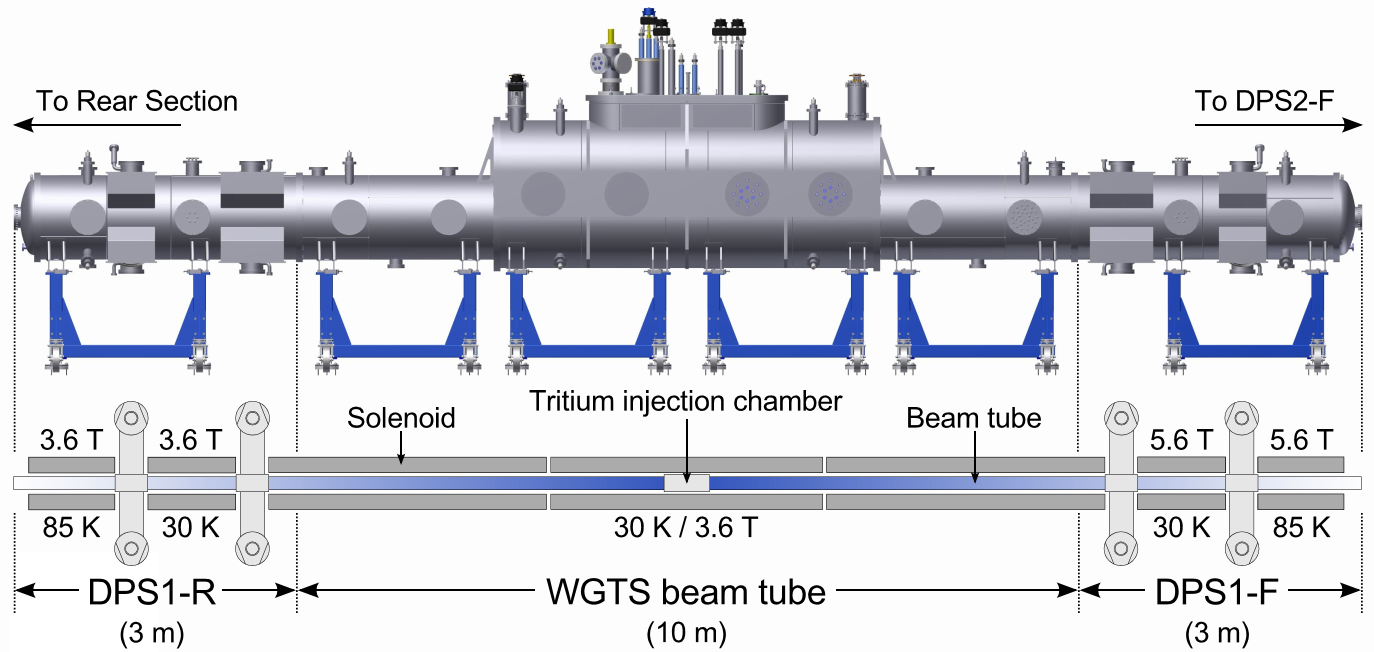
\includegraphics[width=\textwidth]{chapter/katrin/fig/wgts.png}
        \xcaption{KATRIN \glsentryfull{wgts}}{The \glsentryfull{wgts}.}{Shown are the hull and a sketch of the beam tube. Indicated are the molecular pumps, the design temperatures for tritium operation, the maximum magnetic field strengths and a color gradient depicting the decreasing gas density from the center to the sides. (From \cite{Harms2015})}
        \label{fig:wgts}
    \end{figure}%
The \gls{wgts} is a \SI{16}{m}-long, \SI{1.5}{m}-wide and \SI{4}{m}-high cryostat. It is depicted in figure \ref{fig:wgts} and a detailed description can e.g. be found in \cite{Grohman2008}.
    {\par \textbf{The inner loop:} The molecular tritium (\ce{T2}) is injected centrally in the \gls{wgts}'s \SI{90}{mm}-wide beam tube where it decays. The design gas column density is 
    \begin{equation}
        \label{eq:columnDensity}
        \rho d = \SI{5e17}{molecules/{cm}^2}
    \end{equation}
    of which \begin{equation}
        \epsilon_\text{T} = \SI{95}{\percent}
    \end{equation}
    are isotopic tritium molecules. At the front and rear of the \gls{wgts} the gas is extracted from the beam tube by molecular pumps in designated differential pumping sections called DPS-1-R (rear) and DPS-1-F (front). The extracted gas is re-injected in the center of the beam tube. The respective pipe system is called the inner loop.
    \begin{samepage}
    Selected important parts of the inner loop are:
    \begin{itemize}
    \renewcommand{\labelitemi}{$\bullet$}
        \item a buffer vessel where tritium of high purity is introduced from the feed loop of the \gls{tlk};
        \item a \gls{lara} that monitors the isotopic composition of the gas;
        \item a pressure and temperature controlled buffer vessel to regulate the gas inlet into the \gls{wgts}; and
        \item a permeator that separates impurities (like e.g. helium) and ejects them into the exhaust loop of the \gls{tlk}.
    \end{itemize}
    \end{samepage}}
    
    
    {\par\textbf{Magnetic field:}
    In order to adiabatically guide the $\upbeta$ electrons to the spectrometer section the \gls{wgts} is submerged in a magnetic field parallel to its beam tube of up to \SI{5.6}{T}. It is created by 7 superconducting coils, that surround the beam tube. These magnets are kept at a temperature of \SI{4.2}{K} by liquid helium.}
    
    {\par\textbf{Temperature:}
    The stability of the column density \eqref{eq:columnDensity} must be on the \SI{0.1}{\percent} level. This requires stable parameters like temperature $T$ and pressure $p$. On one hand, the higher the temperature the less stable the system. Furthermore, thermal motion smears the energy spectrum of the $\upbeta$ electrons (Doppler effect). On the other hand, at low temperatures the gas molecules cluster. $T=\SI{30}{K}$ is chosen as a compromise and established by a two-phase neon cooling system. For calibration purposes it is also possible to operate the \gls{wgts} with krypton instead of tritium. This requires a beam tube temperature of $T=100K$ in order for the krypton not to freeze. In this operational mode the neon has to be exchanged for argon that provides a suitable vapor pressure.}
    
    \subsection{Rear Section}
    \label{sec:rearSection}
    \begin{figure}[t]
        \inputpdftex{chapter/katrin/fig/rear-section}
    	\xcaption{KATRIN rear section}{The rear section}{terminates the KATRIN beam line and houses several monitoring and calibration devices. (Adapted from \cite{SeitzM2019})}
	    \label{fig:rearSection}
    \end{figure}
    
    The rear section terminates the beam line in the upstream direction. It houses monitoring, calibration and control devices. It is depicted in figure \ref{fig:rearSection} and a detailed description can e.g. be found in \cite{Babutzka2014}.
    
    {\par \textbf{Rear wall:} The so-called rear wall is a gold-coated stainless-steel disc with a diameter of 6 inches that terminates the beam tube.}
    
    {\par\textbf{Electron gun:}
    The rear section houses an electron gun in order to measure the response function of the experiment (see section \ref{sec:response}). Its energy resolution is $\sim \SI{0.2}{eV}$ and its angular resolution is $\sim \SI{4}{\degree}$. The electrons' flight path can be adjusted by dipole magnets mounted in the \gls{wgts} which enables a scanning of the full beam tube.}
    
    {\par\textbf{Plasma control:}
    Space charges, respectively a plasma, forms within the \gls{wgts} due to the tritium decay. $\upbeta$ electrons might therefore start at different potentials which adds uncertainty to the measured $\upbeta$ spectrum. Hence, plasma effects have to be controlled. Simulations show that the plasma can be influenced by the rear wall potential which can be controlled by a voltage supply in the range of $\pm \SI{10}{V}$. Moreover, a UV light illumination of the rear wall can extract electrons via the photoelectric effect that can compensate space charges. Details on the plasma in the \gls{wgts} can e.g. be found in \cite{Kuckert2018}.}
    
    {\par\textbf{Activity monitoring:}
    $\upbeta$ electrons either arrive at the detector or hit the wall of the experiment. A super conducting coil ensures that the magnetic flux tube terminates at the rear wall. On that account, most $\upbeta$ electrons (\SI{99.99}{\percent}) hit the rear wall where they emit bremsstrahlung. Two dedicated \gls{bixs} systems measure the corresponding X-ray spectrum to determine the source strength respectively the gas column density \eqref{eq:columnDensity}.}
    
    \subsection{Differential Pumping Section}
    \label{sec:diffPumpingSection}
    \begin{figure}[t]
        \inputpdftex{chapter/katrin/fig/dps}
    	\xcaption{KATRIN \glsentryfull{dps}}{The \glsentryfull{dps}}{reduces the gas flow and blocks tritium ions. (Adapted from \cite{SeitzM2019})}
	    \label{fig:dps}
    \end{figure}
    The \glsentryfull{dps} is an approximately \SI{5}{m}-long cryostat. It is depicted in figure \ref{fig:dps} and a detailed description can e.g. be found in \cite{Kosmider2012}. In short, it fulfills the following tasks:
    
    {\par\textbf{Reduction of tritium flow:}
    The \glsentryfull{dps} consists of 5 beam tube elements with pump ports between them. The beam tube elements form a \SI{20}{\degree} angle to each other and are arranged in a chicane. While $\upbeta$ electrons are magnetically guided along the chicane, the neutral gas molecules scatter off the walls. This reduces the molecular beaming effect and enhances the pumping probability. Turbo molecular pumps then reduce the gas flow by approximately 5 orders of magnitude and feed the gas into the so-called outer loop where it is reprocessed.}
    
    {\par\textbf{Ion blocking:}
    In the \gls{wgts} ions such as \ce{HeT^+}, \ce{T_2+}, \ce{T_3+}, \ce{T_5+} can form. If not blocked, they reach the spectrometer section analogously to the electrons which would eventually lead to an increased background rate. A potential barrier created by two ring electrodes set to $+\SI{100}{V}$ avoids this. The positive ions are deflected, drift out of the flux tube, hit the wall and get neutralized.}
    
    {\par\textbf{Ion monitoring:}
    Downstream of the blocking electrodes the remaining ion flux is measured by a Fourier transform ion cyclotron resonance device (FT-ICR). Details on ion forming and their measurement can e.g. be found in \cite{Ubieto2009}.}
    
    \subsection{Cryogenic Pumping Section}
    \label{sec:cryoPumpingSection}
    \begin{figure}[t]
        \inputpdftex{chapter/katrin/fig/cps}
    	\xcaption{KATRIN \glsentryfull{cps}}{The \glsentryfull{cps}}{is the coldest part of the KATRIN experiment. Parts of its beam tube a covered by a frozen argon layer at \SI{3}{K} to cold-trap tritium molecules. The low temperatures are established using liquid helium (\ce{LHe}) and an insulation of liquid nitrogen (\ce{LN2}). (Adapted from \cite{SeitzM2019})}
	    \label{fig:cps}
    \end{figure}
    
    The \glsentryfull{cps} is an approximately \SI{7}{m}-long cryostat. It is depicted in figure \ref{fig:cps} and a detailed description can e.g. be found in \cite{Jansen2015}. In short, it fulfills the following tasks:
    {\par\textbf{Reduction of tritium flow:}
    The \gls{cps} consists of 7 beam tube elements of which 5 are arranged in a similar manner as the beam tube elements of the \gls{dps} in a chicane forming \SI{15}{\degree} angles. While charged particles are guided along the chicane by a magnetic field, neutral molecules hit the wall. The walls are covered by a frozen argon layer cooled down to \SI{3}{K} in order to cold-trap particles. After the accumulation of about \SI{1}{Ci} of tritium the argon frost layer has to be renewed. To achieve this the beam tube is warmed-up and the argon is pumped off along with the accumulated tritium. Tests and simulations show a reduction of the tritium flow by approximately 10 orders of magnitude.}

    {\par\textbf{The \glsentryfull{fbm}}: The \glsentryshort{fbm} is a detector that can be moved horizontally into the pump port of the \gls{cps} with a 2-dimensional spacial resolution of \SI{0.1}{mm}. Two pin-diodes measure the $\upbeta$ electron flux and hence, the stability of the column density \eqref{eq:columnDensity}. Furthermore, the \gls{fbm} equips a temperature and a hall sensor. A second detector board holding a Faraday cup for ion measurements is also available. Details on the \gls{fbm} can e.g. be found in \cite{Ellinger2017}.}
    
    {\par\textbf{The \glsentryfull{ckrs}} is a sub mono-layer of \kryptonEightyThree{} on a pyrolytic graphite substrate with a diameter of \SI{2}{cm}. It can be lowered in the pump port of the \gls{cps} and moved in a 2-dimensional plane perpendicular to the beam line. This enables the spacial scanning of the properties of the spectrometer using quasi-monoenergetic conversion electron lines of \kryptonEightyThree. Details on the \glsentryshort{ckrs} can e.g. be found in \cite{Bauer2014}.}
    
    \subsection{Pre and Main Spectrometer}
    \label{sec:spectrometer}
    
    The pre and main spectrometer are vacuum vessels designed to filter passing electrons according to their kinetic energy. The pre spectrometer has a length of \SI{3.4}{m} and a diameter of \SI{1.7}{m}. Details on its design can e.g. be found in \cite{Prall2012}. The main spectrometer has a length of \SI{23}{m} and a diameter of \SI{10}{m}. Details on its design can e.g. be found in \cite{Angrik:2005ep}.
    
    {\par \textbf{\Gls{mace}}: The pre and main spectrometer apply the so-called \glsentryshort{mace} principle. A retarding voltage deflects electrons with insufficient kinetic energy. The electric field gradient is parallel to the beam line, but $\upbeta$ electrons might be emitted in an arbitrary angle. In order to analyze their full kinetic energy they have to be collimated. This is done by a magnetic field gradient. A quantitative description of this process can be found in section \ref{sec:intSpecModel}. The precision of the \gls{mace} principle increases with the size of the spectrometer. That is why the main spectrometer of KATRIN has a larger diameter (\SI{10}{m}) as the the ones of its predecessor experiments.
    }
    
    {\par \textbf{Magnetic field:} The main spectrometer is surrounded by a system of coils that creates the \gls{mace} filter's  magnetic field. Upstream, there is the PS2 magnet; downstream the pinch as well as the detector magnet, which are superconducting solenoids. Their field is fine-tuned by a system of air coils around the spectrometer hull. There is the \gls{emcs} with coils parallel and perpendicular to the beam line axis. Furthermore, there is the \gls{lfcs} with coils perpendicular to the beam line axis. The combined system constrains the electrons' flux tube to the spectrometer vessel and compensates the earth's magnetic field as well as effects from ferromagnetic materials in the spectrometer's surroundings. Details on the magnetic field settings can e.g. be found in \cite{Erhard2018}. Additionally, a vertical and radial magnetic measuring system (\glsentryshort{vmms} and \glsentryshort{rmms}) are installed. The field inside the spectrometer vessel is assessed via samples of these measuring systems combined with simulations. Details on the \glsentryshort{vmms} and the \glsentryshort{rmms} can e.g. be found in \cite{Letnev2018}.}
    
    {\par \textbf{Electric field:} A high voltage system establishes the \gls{mace} filter's retarding potential. According to the KATRIN Design Report \cite{Angrik:2005ep} the retarding voltage's fluctuations must have a standard deviation smaller than \SI{60}{mV} for the envisaged sensitivity on the neutrino mass. The antenna-like beam line setup is sensitive to electromagnetic fluctuations, which is why an active so-called post-regulation system is deployed. It monitors the retarding potential and regulates it with the needed precision. For the monitoring exist the so-called monitor spectrometer and a voltage divider. Details on the voltage calibration with the voltage divider can e.g. be found in \cite{Thuemmler2009}. The monitor spectrometer is part of a second beam line in a separate building. Its retarding potential follows the one one of the main spectrometer and is measured via \kryptonEightyThree{} conversion lines. Details on the monitor spectrometer can be e.g. be found in \cite{Erhard2014}.}
    
    {\par \textbf{Background:} According to the KATRIN Design Report \cite{Angrik:2005ep} the electron rate of uncontrollable sources (background) must be less than \SI{10}{mHz}. Several background-related aspects are:}
    
    {\par \textbf{Vacuum:} The spectrometers are operated at a pressure on the order of \SIrange{10e-11}{10e-12}{mbar}. This prevents electron scattering on residual gas and minimizes background effects by ionization. Correspondingly, several turbo molecular and getter pumps are installed at the spectrometer vessels. Furthermore, the spectrometers can be baked out at up to \SI{350}{\celsius}. Details on the vacuum system can e.g. be found in \cite{Arenz2016}.}
    
    {\par \textbf{Wire electrodes:} The inner walls of the spectrometer vessels are lined by wire electrodes. Their potential is at a few hundred volts below the spectrometer hull reflecting electrons coming from the vessel walls. These electrons might be induced by e.g. cosmic rays or emanate from the spectrometer wall. A detailed description of the wire electrodes can e.g. be found in \cite{Valerius2009}.}
    
    {\par \textbf{Ion blocking:} Analogously to the ones in the \gls{cps} (section \ref{sec:cryoPumpingSection}), three blocking electrodes are installed; one between the \gls{cps} and the pre spectrometer, one between the pre and main spectrometer; and one between the main spectrometer and the detector.}
    
    {\par \textbf{Tandem setup:} $\upbeta$ electrons might scatter on residual gas or the beam line walls. This can either directly lead to secondary electrons or create positive ions that travel down the beam line. The positive ions in turn might again through scattering yield secondary electrons. The more $\upbeta$ electrons enter the main spectrometer the higher is the probability to create secondary electrons. In order to reduce the flux of $\upbeta$ electrons into the main spectrometer the retarding potential of the pre spectrometer is set to a few hundred volts below the one of the main spectrometer. On one hand this is a countermeasure against background events. But on the other hand, charged particles can be trapped between the two spectrometers due to the electromagnetic setup (Penning trap). A sudden discharge might harm the hardware, especially the detector. Therefore, it is possible to sweep a charged wire through the volume in order to collect the trapped particles and avoid this ``Penning-discharges''.}
    
    \subsection{Detector Section}
    \label{sec:detector}
    \begin{figure}[t]
        \inputpdftex{chapter/katrin/fig/detector-section}
    	\xcaption{KATRIN detector section}{The detector section}{terminates the KATRIN beam line. Among other instruments it houses the \glsentrylong{fpd} for $\upbeta$ electrons with the detector wafer at its core.(Adapted from \cite{SeitzM2019})}
	    \label{fig:detector}
    \end{figure}
    
    The detector section terminates the beam line in downstream direction. It can be separated from the spectrometer section by closing a gate valve. The detector section is depicted in figure \ref{fig:detector} and a detailed description can e.g. be found in \cite{Amsbaugh2015}.
    
    {\par \textbf{The \gls{fpd}} counts the $\upbeta$ electrons that pass the spectrometer section. The \gls{fpd} is a pin-silicon detector with a sensitive area of \SI{9}{cm} diameter. It is subdivided in 148 pixels of the same area arranged in 12 rings of 12 pixels each and the so called bull's eye of 4 pixels in the center. This arrangement allows later correction for radial electrical and magnetic inhomogeneities in the beam line.}
    
    {\par \textbf{Shield and veto system:} The \gls{fpd} system's radiation shield consists of two nested cylindrical shells: an outer lead shell of \SI{3}{cm} that reduces photon background and an inner copper shell of \SI{1.27}{cm} that blocks X-rays originating from the outer lead shell. The shield is surrounded by a veto system to tag incoming muons.}
    
    {\par \textbf{Calibration:} Photoelectron sources can be lowered in the detectors line of sight. The corresponding photocurrent can be measured with the so-called \gls{pulcinella} system. A comparison of \gls{pulcinella} and the \gls{fpd} yields the \gls{fpd}'s detection efficiency.}
    
    {\par \textbf{The detector magnet} allows to form the flux tube near the detector independently of the main spectrometer magnetic field setting. This is especially useful in the above mentioned calibration process.}
    
    {\par \textbf{The post-acceleration electrode} allows to shift the energy of $\upbeta$ electrons arriving from the main spectrometer. This way $\upbeta$ electrons can be distinguished from background electrons originating in the detector section by an energy region of interest cut.}
    
   \newcommand{\elecIndex}{\mathrm{e}}
\newcommand{\fermiConst}{G_\mathrm{F}}
\newcommand{\diffRate}{\frac{\d\Gamma}{\d E}}
\newcommand{\nucMatrixElement}{M_\mathrm{nuc}}
\newcommand{\thetaFunc}{\Theta}

\newcommand{\Bsource}{B^j_\mathrm{S}}
\newcommand{\zSource}{z_\mathrm{S}}
\newcommand{\thetaSource}{\theta_\mathrm{S}}
\newcommand{\Esource}{E_\mathrm{S}}
\newcommand{\Usource}{U^j_\mathrm{S}}
\newcommand{\gammaSource}{\gamma_\mathrm{S}}


\newcommand{\Bps}{B_\mathrm{PS2}}
\newcommand{\Bana}{B_\mathrm{A}}
\newcommand{\Bpinch}{B_\mathrm{P}}
\newcommand{\Bmax}{B_\mathrm{max}}
\newcommand{\Bmin}{B_\mathrm{min}}

\newcommand{\thetaMax}{\theta_\mathrm{max}}
\newcommand{\Esur}{E_\mathrm{sur}}
\newcommand{\detEff}{\epsilon_\mathrm{det}}
\newcommand{\macefilterwidth}{\Delta \mathcal{E}^j(\thetaS^j)}

\newcommand{\EtransPure}{E^j_\mathrm{tr}}
\newcommand{\Etrans}{\EtransPure(qU,\Esource,\thetaSource)}
\newcommand{\thetaTransPure}{\theta^j_\mathrm{tr}}
\newcommand{\thetaTrans}{\thetaTransPure(\Esource,qU)}

\newcommand{\As}{A_\mathrm{S}}
\newcommand{\Rbg}{R_\mathrm{bg}}


\section{Modelling of the Integrated \texorpdfstring{$\upbeta$}{Beta} Decay Spectrum with SSC}
\label{sec:intSpecModel}
An analytic description for the electron rate measured by the \gls{fpd} can be derived. The derivation mostly follows \cite{Kleesiek2019, Groh2015, Kleesiek2014} or is extracted from current production code \cite{KATRINCOL2019}. The formulas are implemented in the so-called \gls{ssc} software framework.

\subsection{\texorpdfstring{$\upbeta$}{Beta} Decay Spectrum}
\begin{figure}
    \centering
    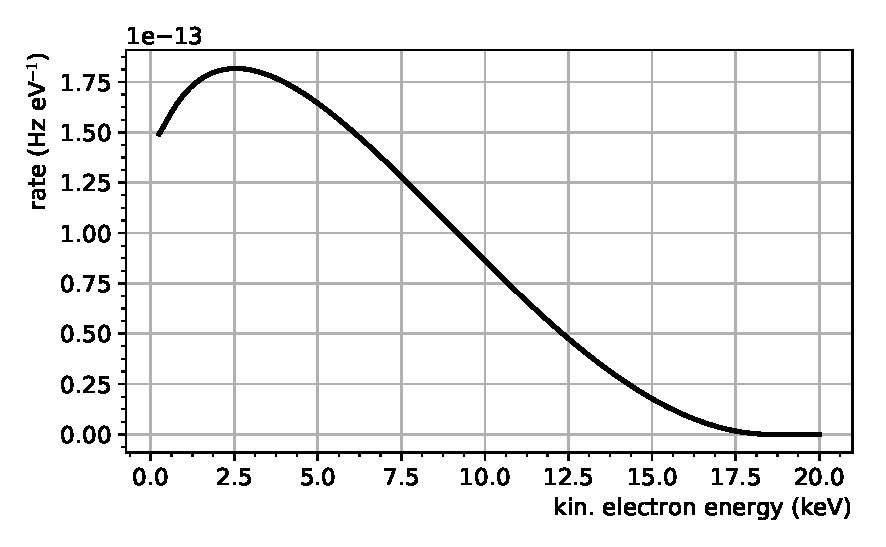
\includegraphics[width=\textwidth]{chapter/katrin/fig/diffSpec.pdf}
    \xcaption{Tritium $\upbeta$ spectrum}{The $\upbeta$ decay spectrum of a tritium molecule}{as calculated by \gls{ssc}.}
    \label{fig:diffSpec}
\end{figure}
\label{sec:diffSpec}
In $\upbeta^-$ decay the released energy is distributed among the emitted electron and the anti-electron neutrino. The differential decay rate of a tritium molecule can be described using Fermi theory and Fermi's golden rule as
\begin{align}
    \label{eq:diffRate}
    \left(\diffRate\right) = &
    \frac{\fermiConst^2 \abs{V_\mathrm{ud}}^2}{2 \pi^3}
    \abs{\nucMatrixElement}^2 \cdot
    F(Z, E) \cdot 
    p(E+m_\elecIndex) \cdot 
    \sum_{f,i} P_f \abs{U_{\elecIndex i}}^2 \epsilon_f \sqrt{\epsilon_f^2-m_i^2} \cdot \thetaFunc(\epsilon_f-m_i)
\end{align}
It is depicted in figure \ref{fig:diffSpec}. Its constituents are the kinetic electron energy $E$;
the PMNS matrix $U$ \eqref{eq:PMNSmatrix}; the neutrino eigenmasses $m_i$ \eqref{eq:nuMassSquared};
the Fermi constant $\fermiConst$;
the up-down-quark-coupling given by the Cabibo angle $\theta_\mathrm{C}$
\begin{equation}
    V_\mathrm{ud} = \cos \theta_\mathrm{C} = 
    0.97425\pm0.00022;
\end{equation}
and the nuclear transition matrix element
\begin{equation}
    \nucMatrixElement = g_V^2+3g_A^2 \quad
    \text{with } g_v = 1 \quad
    \text{and} \quad g_A/g_V = -1.2646 \pm 0.0035
\end{equation}
which is independent of the electron's kinetic energy as the decay is super-allowed and given by the vector $g_V$ and axial vector $g_A$ coupling.

Furthermore, the Fermi function $F(Z,E)$ accounts for the Coulomb interaction between the outgoing electron and the daughter nucleus with atomic charge $Z=2$ which in its relativistic version can be approximated as
\begin{equation}
    F(Z,E) \approx \frac{2 \pi \eta}{1-\exp{2 \pi \eta}} \cdot R \\
\end{equation}
with Sommerfeld parameter $\eta = \alpha Z / \beta$, fine structure constant $\alpha$, relativistic velocity $\beta$ and a relativistic correction factor $R = 1.002037-0.001427\beta$.

The phase-space factor of the outgoing electron with momentum $p$ and mass $m_\elecIndex$ is given by the factor $p(E+m_\elecIndex)$.

The phase space factor of the emitted neutrino is described in dependence of the following quantities: total nuclear tritium decay energy $Q$ (mass difference of mother and daughter nucleus) corrected for the nucleus recoil $E_\mathrm{rec}$ also called endpoint of the $\upbeta$ spectrum
\begin{equation}
    \label{eq:endpoint}
    E_0 = Q-E_\mathrm{rec};
\end{equation}
the kinetic electron energy $E$ and the final state energy of the molecular system $V_f$. The probability that the molecular system is in a final state of energy $V_f$ after the decay is denoted by $P_f$. Then the energy of the neutrino reads 
\begin{equation}
    \epsilon_f = E_0 - E - V_f \fullstop
\end{equation}

The exited energy state $f$ is caused by vibration, rotation or electronic excitation of the decaying molecule. Details and tabulated values can e.g. be found in \cite{Bodine2015} and references therein.

The neutrino's momentum is $\sqrt{\epsilon_f^2-m^2_i}$, where $m_i$ denotes one of the neutrino eigenmasses. The complete phase space factor of the neutrino is a sum over all possible molecular final states labeled $f$ and neutrino eigenmasses labeled $i$.

Lastly, the Heavyside step function $\thetaFunc$ ensures a positive kinetic energy of the neutrino.

\subsection{Detector Counts}
The KATRIN detector counts electrons. The $\upbeta$ electrons are adiabatically guided from the \gls{wgts} to the detector by magnetic fields. The magnetic field lines are parallel to the beam line axis. The angle between the flight direction of a $\upbeta$ electron and the beam line axis towards the detector is denoted by the pitch angle $\theta \in [\SI{0}{\degree}, \SI{180}{\degree}]$. The starting position of an $\upbeta$ electron is denoted by its 1-dimensional coordinate along the beam line axis $\zSource$. 

KATRIN measures an integrated $\upbeta$ spectrum. In other words, the detector counts electrons of kinetic energy $\Esource$ above a threshold, the so-called retarding energy $qU$. The integrated $\upbeta$ spectrum can be scanned by varying $qU$.

A $\upbeta$ electron emitted in the \gls{wgts} reaches the detector with a probability modeled by the so-called response function $R$ (see section \ref{sec:response}). $R$ depends on the experimental settings (such as the electromagnetic fields and the gas dynamics) and especially on the retarding energy $qU$. Here, $R$ denotes the transmission probability for a $\upbeta$ electron of a fixed starting kinetic energy $\Esource$, starting position $\zSource$ and starting pitch angle $\thetaSource$. The probability of a $\upbeta$ electron for being counted when reaching the detector is denoted by the detection efficiency $\detEff$. Furthermore, the number of tritium molecules in the \gls{wgts} in a small area around the coordinate $z$ is denoted by $\d N_T(z)$. 

Then, the measured integrated rate is expressed as integral from the threshold energy $qU$ to the endpoint energy $E_0$ \eqref{eq:endpoint} over the differential rate $\d \Gamma / \d \Esource$ \eqref{eq:diffRate} weighted with the probability given by $R$ as
\begin{equation}
\label{eq:rateDependingOnstartingValues}
\Gamma(qU, \zSource, \thetaSource) = 
\detEff \cdot
\d N_T(\zSource) \cdot
\int_{qU}^{E_0} 
    \left(\frac{\d \Gamma(\Esource)}{\d \Esource}\right) \cdot 
    R(\Esource, qU, \zSource, \thetaSource) 
\d \Esource
\comma
\end{equation}
which eventually leads to $\upbeta$ electron counts by multiplication with the measurement time $t(qU)$ at a retarding energy $qU$
\begin{equation}
    \label{eq:countsDependingOnPositionAndPitchAngle}
    N(qU, \zSource, \thetaSource) = \Gamma(qU, \zSource, \thetaSource) \cdot t(qU)
    \fullstop
\end{equation}

\subsection{Discretization of the \glsentryshort{wgts} Volume}
\label{sec:sourceDiscretization}
The counts $N$ \eqref{eq:countsDependingOnPositionAndPitchAngle} are given for $\upbeta$ electrons of a fixed starting position $\zSource$.
All starting positions $\zSource \in [-L/2, +L/2]$ within the \gls{wgts} of length $L$ contribute to the total count rate at the detector. Integrating along the beam axis accounts for this
\begin{equation}
    N(qU, \thetaSource) = \int_{-L/2}^{+L/2} \frac{\d N(qU, \thetaSource, \zSource)}{\d \zSource} \d \zSource
\end{equation}
Numerically, the same result can be obtained by a sufficiently fine discretization of the \gls{wgts} volume into $S$ slices. The counts $N$ \eqref{eq:countsDependingOnPositionAndPitchAngle} are adapted accordingly to account for discrete starting $\upbeta$ electron positions $\zSource^j$
\begin{equation}
    N(qU, \thetaSource, \zSource) \rightarrow N^j(qU, \thetaSource,\zSource^j) \equiv N^j(qU, \thetaSource) \fullstop
\end{equation}
Then, the total counts read
\begin{equation}
    \label{eq:nonAveragedCounts}
    N(qU, \thetaSource) = \sum_{j=1}^S N^j(qU, \thetaSource) \fullstop
\end{equation}
Within this chapter, from here forth all quantities that are subject to discretization will be labeled with an upper index $j$. The discretization especially propagates to the response function $R \rightarrow R^j$ and its constituents.

\subsection{Magnetic Bottle Effect}
The $\upbeta$ electrons are adiabatically guided to the detector by magnetic fields. The magnetic field strength at the starting position of a $\upbeta$ electron in the \gls{wgts} is denoted by $\Bsource$. The maximum magnetic field strength along the beam line is denoted by $\Bmax$. As $\Bsource<\Bmax$ $\upbeta$ electrons travelling downstream to the detector are subject to the magnetic bottle effect. They get reflected and travel upstream to the rear wall if their starting pitch angle $\thetaSource$ surpasses $\thetaMax^j$ with
\begin{equation}
    \label{eq:thetaMax}
    \sin\thetaMax^j = \sqrt{\frac{\Bsource}{\Bmax}} \fullstop
\end{equation}
(Its KATRIN design value is $\thetaMax\approx \SI{51}{\degree}$.) A cutting angle $\thetaMax^j$ is beneficial because the greater the emission angle of a $\upbeta$ electron the larger the distance it travels in the \gls{wgts} and the more it is subject to energy losses such as scattering or synchrotron radiation.

\subsection{Scattering Probabilities}
\label{sec:scatProbs}
The probability for a $\upbeta$ electron to reach the detector (the response function $R^j$) depends on the scattering probabilities $P_l$ ($l \in \NN$). $P_l$ denotes the probability of an electron to scatter $l$ times when travelling through the \gls{wgts}. $P_l$ depends on the starting position $\zSource$ of a $\upbeta$ electron in the \gls{wgts} as well as on its starting pitch angle $\thetaSource$. The expected scattering count for a $\upbeta$ electron when travelling through the \gls{wgts} is the product of the line density $\lambda$ the electron passes through and the scattering cross section $\sigma$
\begin{equation}
    \label{eq:expectedScatteringCount}
    \mu(\zSource, \thetaSource) = \lambda(\zSource,\thetaSource) \sigma \fullstop
\end{equation}
The electron moves on a spiral due to its cyclotron motion. Therefore, when traveling an infinitesimal distance $\d z$ in $z$-direction, it travels a total distance of
\begin{equation}
    \label{eq:infinitesimalElecPath}
    \d s = \frac{1}{\cos\thetaSource} \d z \fullstop
\end{equation}
The line density $\lambda$ can be expressed as a line integral over the gas density $\rho$ along the electrons path $\varphi$
\begin{equation}
    \label{eq:lambdaPath}
    \lambda(\zSource,\thetaSource) = \int_{\varphi} \rho(\Vec{r})\d s
    \fullstop
\end{equation}
Assuming that the gas density $\rho$ only depends on the $z$-position along the beam line and vanishes for $z>L/2$ (beyond the \gls{wgts}) equation (\ref{eq:lambdaPath}) becomes
\begin{equation}
    \label{eq:lambdaPathIntegral}
    \lambda(\zSource,\thetaSource) = \frac{1}{\cos\thetaSource}\int_{\zSource}^{L/2} \rho(z)\d z \fullstop
\end{equation}
Hence, the expected scattering count (\ref{eq:expectedScatteringCount}) becomes
\begin{equation}
    \label{eq:expectedScatRate}
    \mu(\zSource, \thetaSource) = \frac{\sigma}{\cos\thetaSource}\int_{\zSource}^{L/2} \rho(z)\d z \fullstop
\end{equation}
The scattering process fulfills the conditions of a Poisson process, namely scattering once does quasi not influence the probability of an electron to scatter again; the expected scattering count $\mu$ \eqref{eq:expectedScatRate} stays quasi constant; and it is unlikely for two scatterings to happen within a short distance. Thus, the probability for $l$-fold scattering can be expressed as a Poisson distribution
\begin{equation}
    \label{eq:scatProbs}
    P_l(\zSource, \thetaSource) = 
    \frac{
        \mu(\zSource, \thetaSource)^l
    }{l!}
    \mathrm{e}^{-\mu(\zSource, \thetaSource)} \fullstop
\end{equation}
\paragraph{Discretization of the \gls{wgts} volume}
In the discretized case the \gls{wgts} volume is divided into $S$ slices indexed by $k$ with an average gas density $\bar{\rho}^k$. A slice $k$ starts at position $Z_s^k$ and ends at position $Z_e^k$ with a width of $W^k=Z_e^k-Z_s^k$. For $\upbeta$ electrons that start at a position $z$ within slice $j$ the expected scattering count \eqref{eq:expectedScatteringCount} becomes
\begin{equation}
\label{eq:nonAveragedExpectedScatCount}
    \mu(\zSource, \thetaSource) \rightarrow 
    \mu^j(z, \thetaSource) =
    \frac{\sigma}{\cos\thetaSource}
    \underbrace{
        (Z_e^j-z) \bar{\rho}^j
        \vphantom{\sum_{k=j+1}^{S}}
    }_{(*)}
    \underbrace{\sum_{k=j+1}^{S} \bar{\rho}^k W^k}_{(**)}
    \fullstop
\end{equation}
The gas column density in front of a $\upbeta$ electron is split in two parts: the slice of its \mbox{origin $(*)$} and all slices downstream \mbox{$(**)$}. 

The Poisson distribution is formed for the expected scattering count $\mu^j$ \eqref{eq:nonAveragedExpectedScatCount} and averaged over all starting positions within the slice $j$ which yields the discretized scattering probabilities
\begin{equation}
    \label{eq:nonAveragedScatProbs}
    P^j_l(\thetaSource) = 
    \frac{1}{W^j}
    \int_{Z_s^j}^{Z_e^j}
        \frac{
            \left(\mu^j(z,\thetaSource)\right)^l
        }{l!}
        \mathrm{e}^{-\mu^j(z,\thetaSource)}
    \d z
    \fullstop
\end{equation}


\subsection{\glsentryshort{mace} Principle and Transmission Function}
\label{sec:mace}
\begin{figure}[t]
        \inputpdftex{chapter/katrin/fig/mace}
    	\xcaption{Schematic of the KATRIN main spectrometer and the \glsentryshort{mace} principle.}{
    	Schematic of the KATRIN main spectrometer and the \glsentryfull{mace} principle.}{
    	 The {KATRIN} design magnetic field settings are
    	$\Bps=\SI{4.5}{T}$, 
    	$\Bsource=\SI{3.6}{T}$, 
    	$\Bmax=\SI{6.0}{T}$, 
    	$B_\mathrm{D}=\SI{3.6}{T}$, 
    	$\Bana\approx\SI{3e-4}{T}$. $\Vec{E}$ denotes the magnetic field regulated by the retarding potential $U$ that reaches its maximum $U_\mathrm{a} = U$ at the analyzing plane. (Adapted from \cite{SeitzM2019})
    	}
	    \label{fig:mace}
    \end{figure}

The spectrometers of KATRIN follow the \glsentryfull{mace} principle. Figure \ref{fig:mace} shows a corresponding sketch. The main spectrometer is a vacuum vessel with a downstream magnet of strength $\Bps$ and an upstream magnet of strength $\Bpinch$ making electrons form a magnetic flux tube. In the case of KATRIN the fluxtube begins in the \gls{sts} with a magnetic field strength of $\Bsource$. In other words, the spectroscopic properties are not solely determined by the spectrometer vessel, but also by the \gls{sts}. The minimum magnetic field strength $\Bmin = \Bana$ is reached at the so-called analyzing plane in the vessel center. Electrons entering the vessel perform cyclotron motions around the magnetic field lines. Their total kinetic energy $\Esource$ is split into a longitudinal component $E_\parallel$ along the beam axis and a transverse component $E_\bot$
\begin{equation}
    \label{eq:totalKinElecEnergy}
    \Esource = E_\parallel + E_\bot \fullstop
\end{equation}
In the non-relativistic and adiabatic approximation the transverse component can be expressed by the magnetic field strength $B$ and the electron's magnetic moment $\mu$ respectively its charge $q=e$, its mass $m_\elecIndex$ and angular momentum $L$.
\begin{equation}
    E_\bot = - \mu B = \frac{e}{2 m_\elecIndex}LB \fullstop
\end{equation}
Adiabaticity conserves angular momentum $L$ and the total energy of the electron $\Esource$. Hence, when the magnetic field strength $B$ decreases to $\Bana=\Bmin$ in the analyzing plane, the transverse component of the electron's energy $E_\bot$ decreases likewise and transforms to longitudinal energy $E_\parallel$. Additionally, a retarding voltage barrier is applied along the beam axis, reaching its maximum $U$ at the analyzing plane and dropping of towards the source and the detector. 
In order to pass through the filter, electrons need a total kinetic energy $\Esource$ greater than the transmission energy $\Etrans$ that depends on their starting potential $\Usource$, their starting pitch angle $\thetaSource$ and starting Lorentz factor $\gammaSource$
\begin{equation}
    \label{eq:transmissionEnergy}
    \Etrans = 
    \frac{
        q(U-\Usource)
    }{
        1-\sin^2\thetaSource \frac{\Bana}{\Bsource} \frac{\gammaSource+1}{2}
    }
    \fullstop
\end{equation}
For ease of notation, the dependency on $\Bsource$, $\Bana$ and $\Usource$ is left implicit. Note further that the right hand side of \eqref{eq:transmissionEnergy} also depends on the starting energy of a $\upbeta$ electron as it depends on $\gammaSource$.

Then, the probability for an electron to pass through a \gls{mace} filter, the so-called transmission function, can be written as
\begin{equation}
    \label{eq:transmissionWithConditionOnEnergy}
    \mathcal{T}^j(\Esource, qU, \thetaSource) =
    \begin{cases}
    1 & \text{if } \Esource > \Etrans \\
    0 & \text{otherwise} 
    \end{cases}
    \fullstop
\end{equation}

The transmission condition for the energy $\Esource > \Etrans$ can be reformulated to a condition for the pitch angle $\thetaSource^j$
\begin{align}
    \label{eq:transmissionPitchAngle}
    &\Esource > \Etrans \\
    \Leftrightarrow \quad
    & \thetaSource < \thetaTrans
    \coloneqq
    \arcsin
    \left(\sqrt{
        \frac{\Esource-q(U-\Usource)}{\Esource} 
        \frac{\Bana}{\Bsource}
        \frac{\gammaSource+1}{2}
    }\right)
\end{align}
This allows to rewrite the transmission function \eqref{eq:transmissionWithConditionOnEnergy} as
\begin{equation}
    \label{eq:transmission}
    \mathcal{T}^j(\Esource, qU, \thetaSource) =
    \begin{cases}
    1 & \text{if } \thetaSource > \thetaTrans \\
    0 & \text{otherwise} 
    \end{cases}
    \fullstop
\end{equation}

\subsection{Response Function}
\label{sec:response}
The so-called response function denotes the probability of a $\upbeta$ electron emitted in the \gls{wgts} with starting energy $\Esource$ and pitch angle $\thetaSource$ to reach the detector when a retarding voltage of $U$ is applied to the spectrometer. In addition to the transmission function $\mathcal{T}^j$ \eqref{eq:transmissionPitchAngle} it incorporates the energy loss $\epsilon$ of the $\upbeta$ electrons due to scattering in the gas in the \gls{wgts}. If up to $N$-fold scattering is considered, the response function reads
\begin{equation}
    \label{eq:nonAveragedResponse}
    R^j(\Esource, qU, \thetaSource) = 
    \int_0^{\Esource}
        \sum_{l=1}^{N}
            \mathcal{T}^j(\Esource-\epsilon, qU, \thetaSource) \cdot
            P^j_l(\thetaSource) \cdot f_l(\epsilon)
    \d \epsilon
    \fullstop
\end{equation}
Here, $P^j_l$ \eqref{eq:nonAveragedScatProbs} denotes the probability of a $\upbeta$ electron to scatter $l$ times when travelling through the \gls{wgts}. $f_l(\epsilon)$ is the so-called energy loss function. It denotes the probability for $\upbeta$ electrons to loose the energy $\epsilon$ when scattering $l$ times. For no scattering the Dirac delta function is used
\begin{equation}
    f_0(\epsilon) = \delta(\epsilon) \fullstop
\end{equation}
For $1$-fold scattering $f_1$ is denoted without index $f_1 = f$. For $l>1$ and $l$-fold scattering $f_l$ is the $l$-fold convolution of $f$ with itself
\begin{equation}
    f_l(\epsilon) = \Conv_{i=1}^{l} f(\epsilon)
\end{equation}
where $\conv$ denotes the convolution
\begin{equation}
    (f \conv f)(\epsilon) = \int_{0}^{\infty}  f(\epsilon-\epsilon^\prime)f(\epsilon^\prime) \d \epsilon^\prime \fullstop 
\end{equation}

\subsection{Energy Loss Function}
\label{sec:eloss}
The response function \eqref{eq:nonAveragedResponse} depends on the energy loss function $f$. $f(\epsilon)$ denotes the probability of a $\upbeta$ electron to loose the energy $\epsilon$ when scattering once on a gas molecule. A review of different models for $f$ can e.g. be found in \cite{Trost2019}. E.g. a phenomenological model fitted to data was established by the Troitsk experiment for tritium \cite{Aseev2000} as well as for deuterium and hydrogen molecules \cite{Abdurashitov2017}. Currently a corresponding  modeling effort is made based on data taken by KATRIN. Details will be discussed in section \ref{sec:elossSensitivity}.

\subsection{Distribution of Pitch Angles}
\label{sec:pitchAngleAveraging}
The detected counts $N$ (\ref{eq:nonAveragedCounts}) are given for a fixed starting pitch angle $\thetaSource$ of $\upbeta$ electrons which motivates to average over pitch angles. Any function $g(\thetaSource)$ depending on a fixed pitch angle $\thetaSource$ can be averaged given the distribution $\omega(\thetaSource)$ of $\thetaSource$ and its maximum value $\thetaMax^j$ \eqref{eq:thetaMax} as
\begin{equation}
    \label{eq:pitchAngleAveraging}
    \langle g(\thetaSource) \rangle \equiv \bar{g} =  
    \frac{
        \int_{0}^{\thetaMax^j} 
            \omega(\thetaSource)
            g(\thetaSource)
        \d \thetaSource   
    }{
        \int_{0}^{\thetaMax^j} 
            \omega(\thetaSource)
        \d \thetaSource 
    } \fullstop
\end{equation}
An isotropic $\upbeta$ electron emission by a tritium molecule into the unit sphere, meaning all combinations of spherical emission angles $(\varphi, \vartheta=\thetaSource)$ are equally likely, yields as distribution for their starting pitch angle
\begin{align}
    \omega(\thetaSource) &= \sin\thetaSource \\
    \int_{0}^{\thetaMax^j} 
            \omega(\thetaSource)
        \d \thetaSource 
    &= \frac{1}{1-\cos\thetaMax^j}
    \fullstop
\end{align}

\paragraph{Scattering Probabilities}
Averaging the scattering probabilities $P_l^j$ \eqref{eq:nonAveragedScatProbs} yields
\begin{equation}
    \label{eq:averagedScatProbs}
        \bar{P}_l^j = \frac{1}{1-\cos\thetaMax^j} \int_{0}^{\thetaMax^j} P_l^j(\thetaSource) \sin\thetaSource \d \thetaSource \fullstop
\end{equation}
This expression is helpful when averaging the detected counts $N$ \eqref{eq:nonAveragedCounts} and bringing the corresponding averaged response function in a demonstrative form as shown below.

\paragraph{Counts and Response Function}
\begin{figure}
    \centering
    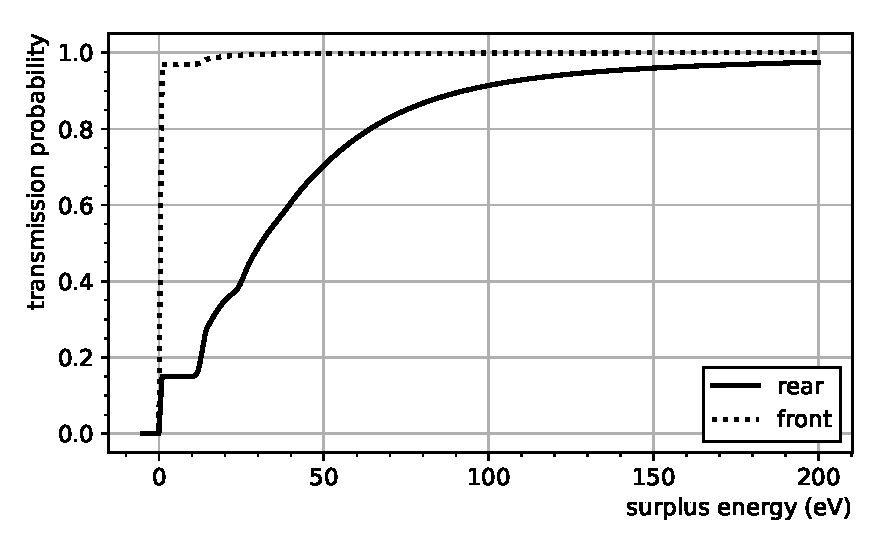
\includegraphics[width=\textwidth]{chapter/katrin/fig/response.pdf}
    \xcaption{KATRIN response function}{The response function}{as calculated by \gls{ssc}. The surplus energy denotes the difference between the starting kinetic energy $\Esource$ of a $\upbeta$ electron and the retarding energy $qU$. The response function $\bar{R}^j$ \eqref{eq:SSCresponse} is depicted for electrons starting at the rear and front of the \gls{wgts}.}
    \label{fig:response}
\end{figure}
The detected counts $N$ \eqref{eq:nonAveragedCounts} depend on the starting pitch angle $\thetaSource$ of the $\upbeta$ electrons. They have to be averaged over $\thetaSource$. The corresponding integral can be swapped with the sum over the \gls{wgts} slices and the integral over the energy and propagates to the response term
\begin{align}
\label{eq:SSCcounts}
\bar{N}(qU) \propto \sum_{j=1}^S N_T^j
\int_{qU}^{E_0}
    \left(\frac{\d \Gamma(\Esource)}{ \d \Esource}\right) \cdot
    \frac{1}{1-\cos\thetaMax^j}
    \int_{0}^{\thetaMax^j}
        R^j(\Esource, qU, \thetaSource) 
        \sin\thetaSource \d \thetaSource
\d \Esource
\fullstop
\end{align}
Here $N_T^j$ denotes the number of tritium molecules in a \gls{wgts} slice $j$. The response function $R^j$ (\ref{eq:nonAveragedResponse}) can be averaged as
\begin{equation}
\begin{split}
    \bar{R}^j(\Esource,qU) &= 
    \frac{1}{1-\cos\thetaMax^j}
    \int_{0}^{\thetaMax^j}
        R^j(\Esource, qU, \thetaSource) 
    \sin\thetaSource \d \thetaSource \\ &=
    \int_0^{\Esource}
        \sum_{l=1}^{N}
            \frac{1}{1-\cos\thetaMax^j}
            \int_{0}^{\thetaMax^j}
            \mathcal{T}^j(\Esource-\epsilon, qU, \thetaSource) \cdot
            P^j_l(\thetaSource)
            \sin\thetaSource \d \thetaSource
            f_l(\epsilon)
    \d \epsilon
    \fullstop
\end{split}
\end{equation}
The transmission function $\mathcal{T}^j$ \eqref{eq:transmission} is a step function. Assuming that $\thetaMax^j$ \eqref{eq:thetaMax} is always greater than the transmission angle $\thetaTransPure$ \eqref{eq:transmissionPitchAngle}, the upper integral boundary changes which yields the averaged response function
\begin{equation}
    \label{eq:slimResponse}
    \bar{R}^j(\Esource, qU) =
    \int_0^{\Esource}
        \sum_{l=1}^{N}
            \int_{0}^{\thetaTransPure(\Esource-\epsilon, qU)}
            \frac{
                \sin\thetaSource \cdot P^j_l(\thetaSource)
            }{
                1-\cos\thetaMax^j
            }
            \d \thetaSource
            f_l(\epsilon)
    \d \epsilon
    \fullstop
\end{equation}
The averaged response function $\bar{R}^j$ is depicted in figure \ref{fig:response}. Its formula \eqref{eq:slimResponse} can be rewritten to match the form of the formula for the non-averaged response function \mbox{$R^j$ \eqref{eq:nonAveragedResponse}}. Therefore, the averaged scattering probabilities $\bar{P}^j_l$ \eqref{eq:averagedScatProbs} are used and the factor $1 = \bar{P}^j_l / \bar{P}^j_l$ is inserted in equation \eqref{eq:slimResponse}:
\begin{align}
    \label{eq:implementedResponse}
    \bar{R}^j(\Esource, qU) &=
    \int_0^{\Esource}
        \sum_{l=1}^{N}
            \underbrace{
                \int_{0}^{\thetaTransPure(\Esource-\epsilon, qU)}
                \frac{
                    \sin\thetaSource \cdot P^j_l(\thetaSource)
                }{
                    (1-\cos\thetaMax^j) \cdot \bar{P}^j_l
                }
                \d \thetaSource
            }_{
                T^{j,\star}(\Esource-\epsilon, qU)
            } \cdot 
            \bar{P}^j_l \cdot
            f_l(\epsilon)
    \d \epsilon \\ &=
    \int_0^{\Esource}
        \sum_{l=1}^{N}
            T^{j,\star}(\Esource-\epsilon, qU) \cdot 
            \bar{P}^j_l \cdot
            f_l(\epsilon)
    \d \epsilon
    \label{eq:SSCresponse}
    \fullstop
\end{align}
Note that the non-averaged response function $R^j$ \eqref{eq:nonAveragedResponse} has the same form as the averaged one $\bar{R}^j$ \eqref{eq:SSCresponse} if the non-averaged transmission function $\mathcal{T}^j$ \eqref{eq:transmission} is replaced by the modified transmission function $T^{j,\star}$ and the non-averaged scattering probabilities $P^j_l$ (\ref{eq:scatProbs}) by the averaged ones $\bar{P}^j_l$ \eqref{eq:averagedScatProbs}.

Note further that albeit equation (\ref{eq:slimResponse}) and equation (\ref{eq:SSCresponse}) are analytically equal, they are not equal implementation-wise. Currently the implementation of the response function follows equation (\ref{eq:SSCresponse}). One one hand, equation (\ref{eq:slimResponse}) is more ``light-weight'' as it does not use the averaged scattering probabilities. In the future it might be beneficial to alter the implementation to simplify the program structure and cut down on the number of calculations. On the other hand, equation \eqref{eq:implementedResponse} allows the exchange of implementations for the transmission function whereas equation \eqref{eq:slimResponse} only allows to exchange the implementation of the response function as a whole.

\subsection{Reconciliation}
The predicted counts for a retarding energy of $qU$ when measuring a duration $t(qU)$ are
\begin{equation}
	\label{eq:countsSCCFinal}
	\bar{N}(qU) = t(qU) \cdot \detEff \cdot \left(
		\As \cdot
		 \sum_{j}
			N_T^j \cdot
			\int_{qU}^{E_0} 
				\left(\frac{\d \Gamma(\Esource)}{ \d \Esource}\right) \cdot 
				\bar{R}^j(\Esource, qU) 
			\d \Esource +
			\Rbg
		\right)
	\fullstop
\end{equation}
Here, $\As=1$ is a normalization factor, $\detEff \in [0,1]$ the detector efficiency, the sum goes over all source slices, $N_T^j$ is the number of tritium molecules in the $j$th source slice, $\left(\d \Gamma(\Esource) / \d \Esource \right)$ is the differential rate from \eqref{eq:diffRate}, $\bar{R}^j(\Esource, qU)$ is the response function from \eqref{eq:SSCresponse} and $\Rbg$ is the rate of background events.

\subsection{Amendments}
Equation \eqref{eq:countsSCCFinal} is a scaffold for an analytic model of the counts measured by the KATRIN detector. Modifications of isolated terms can consider further effects. Selected examples are:
\begin{itemize}
    \item \textbf{Doppler effect:} Gas flow and temperature move the tritium molecules and hence, smear the kinetic energy distribution of $\upbeta$ electrons. This can be modelled by convolving the differential rate $\d \Gamma / \d E$ \eqref{eq:diffRate} with a Maxwellian distribution or by applying corrections to the final energy states of the decaying molecules.
    \item \textbf{Plasma potential:} Space charges, respectively a plasma, forms within the \gls{wgts} due to the tritium decay. Electrons passing through space charges might either gain or loose energy. In a segmented \gls{wgts} volume, this is implemented by using an effective retarding energy corrected for the plasma potential $V^j$ in the slice $j$
    \begin{equation}
        qU \rightarrow qU^j_\mathrm{eff} = qU - V^j
    \end{equation} 
    when calculating the response function $\bar{R}^j$ \eqref{eq:SSCresponse}. Note that this is equivalent to using the starting potential $\Usource$ in the transmission energy $\EtransPure$ \eqref{eq:transmissionEnergy}.
    \item \textbf{Further discretization of the \gls{wgts} volume:} The \gls{ssc} software allows to discretize the \gls{wgts} not only into slices, but also to subdivide the slices further into rings and the rings into segments. This enables an arbitrary spacial binning for \gls{wgts} properties such as the magnetic field or gas density. Then, additionally, the retarding energy $qU \rightarrow qU^j$, the maximum magnetic field strength  along the beam line $\Bmax \rightarrow \Bmax^j$, the magnetic field strength in the analyzing plane $\Bana \rightarrow \Bana^j$ and the detector efficiency $\epsilon_\mathrm{det} \rightarrow \epsilon_\mathrm{det}^j$ become subject to discretization because they exhibit a radial dependency. Furthermore, the \gls{wgts} can be subdivided into volumes that map onto a specific detector pixel due to magentic guidance. This enables pixel-wise modelling of electron counts.
\end{itemize}
    \def\currentRootFolder{chapter/energyDependentCrossSec}
\def\currentFigureFolder{\currentRootFolder/fig}
\newcommand{\sigmaInel}{\sigma_\mathrm{inel}}
\newcommand{\sigmaAvg}{\sigma_\mathrm{avg}}

\newcommand{\qUmin}{qU_\mathrm{min}}

\newcommand{\Ekin}{E_\mathrm{kin}}
\newcommand{\nSource}{n_\mathrm{S}}
\newacronym{standardmodel}{SM}{Standard Model of Particle Physics}
\newacronym{lep}{LEP}{Large Electron Positron Collider}
\newacronym{ssm}{SSM}{standard solar model}
\chapter{Energy-Dependence of the Cross Section for Inelastic Electron-Scattering within the \glsentryshort{wgts}}
\label{sec:eDepScatCrossSec}
The probability of an electron to scatter when traveling through the \gls{wgts} can be characterized by the total scattering cross section $\sigma_\mathrm{tot}$. Two types of scatterings can be distinguished: elastic and inelastic scattering. The cross section for elastic scattering is smaller than the one for inelastic scattering by one order of magnitude~\cite{Kleesiek2019}. This chapter focuses on inelastic scattering and neglects elastic scattering. Within this chapter, the cross section for electrons scattering inelastically off tritium molecules is just denoted as ``cross section'' and with the symbol $\sigma$. For ease of notation and reading, the adjective ``inelastic'' and an index such as ``inel'' is omitted where the context allows it unambiguously.

The cross section depends on the energy of the incident electrons: $\sigma \equiv \sigma(E)$. This dependence has been neglected in the formal modeling of a KATRIN measurement described in chapter~\ref{sec:intSpecModel}. This chapter investigates effects related to the incorporation of the energy-dependence. Section~\ref{sec:eDepScatCrossSecSources} lists cross section values and formulae from different sources and relates them to each other. Section~\ref{sec:eDepScatCrossSecModelPoisson} extends the mathematical formalism for a KATRIN measurement in order to incorporate the energy-dependence of the scattering cross section. However, an approximation is made. It is neglected, that an electron that scatters loses energy and becomes more likely to scatter again. This issue is addressed in section~\ref{sec:eDepScatCrossSecModelExtended}. Section~\ref{sec:eDepScatCrossSecNuMassInf} discusses the energy-dependence of the scattering cross section within the context of neutrino mass inference using the approximated model. And section~\ref{sec:eDepScatCrossSecConclusion} concludes and offers an outlook.


\section{Cross Section for Electrons Scattering off Molecular Hydrogen Isotopologues}
\label{sec:eDepScatCrossSecSources}
The goal of this thesis is to investigate to what extend it is important, that the cross section value is not constant but varies with the energy of the incident electrons. In that regard, a formula by~\cite{Liu1987} is used, that is derived from first principles and denotes the energy-dependent cross section for electrons scattering off hydrogen molecules. This was found to be a feasible approach for the stated goal - at least for first investigations. In section~\ref{sec:eDepScatCrossSecSourcesTheory}, this formula by~\cite{Liu1987} is reviewed. For electrons with an energy of $\Esource=\SI{18.6}{keV}$, its application yields 
\begin{equation}
	\label{eq:eDepScatCrossSecSourcesCrossSecLiuAtEndpoint}
	\sigma(\SI{18.6}{keV}) = \SI{3.667e-22}{m^2}
	\fullstop
\end{equation}
The formula is in agreement on at least the $10^{-1}$ level with recent, preliminary estimations obtained through data taken at the KATRIN experiment for electrons scattering off tritium molecules. This hints at its applicability, which is of importance in the light of the following paragraph.

The situation regarding cross section values is not without a certain intricacy. The following list gives an introduction to the matter that shall serve as guidance for the reader:\mynobreakpar
\begin{enumerate}
	\item In this work, a theoretical cross section for electrons scattering off hydrogen molecules is used. During a KATRIN neutrino mass measurement, the \gls{wgts} is envisaged to be filled with gas of \SI{95}{\percent} tritium purity~\cite{Angrik:2005ep}. In that regard, the scattering off tritium molecules is of importance with respect to the KATRIN experiment. How the formulas for scattering off hydrogen molecules can be transformed to tritium molecules is under investigation at the time of writing this thesis. Once, this process is completed, the study presented in this thesis might have to be repeated.
	\item The cross section for electrons with an energy of \SI{18.6}{keV} scattering off tritium molecules was measured at the neutrino mass experiment in Troitsk to be~\cite{Aseev2000}
	\begin{equation}
		\sigma(\SI{18.6}{eV}) = \SI{3.40\pm0.07e-22}{m^2}
		\fullstop
	\end{equation}
	This value differs by approximately \SI{8}{\percent} and 4 standard deviations from the theoretical value given above in equation~\eqref{eq:eDepScatCrossSecSourcesCrossSecLiuAtEndpoint}.
	\item The KATRIN Design Report lists a reference value~\cite{Angrik:2005ep}
	\begin{equation}
	\label{eq:eDepScatCrossSecSourcesCrossSecTDR}
	\sigma_\mathrm{TDR} = \SI{3.456e-22}{m^2}
	\fullstop
	\end{equation}
	This value also differs significantly from the theoretical value given above in equation~\eqref{eq:eDepScatCrossSecSourcesCrossSecLiuAtEndpoint}. To further complicate the matter, comparability with former results is of importance in the scope of this thesis and several former works are based on $\sigma_\mathrm{TDR}$. Section~\ref{sec:eDepScatCrossSecSourcesChoice} explains why the value of $\sigma_\mathrm{TDR}$ might be erroneous and how this issue is addressed in this work.
\end{enumerate}

\subsection{Theoretical Cross Section Formulae}
\label{sec:eDepScatCrossSecSourcesTheory}
An expression for the inelastic cross section for electrons scattering off hydrogen molecules can be found in~\cite{Liu1973}. Two expressions are given: one for relativistic incident electrons and one for non-relativistic incident electrons. In regard to KATRIN, the energies of $\upbeta$~electrons from tritium $\upbeta$~decay are relevant. The maximum relativistic $\beta$~factor of electrons from tritium $\upbeta$~decay is
\begin{align}
\beta(E, m) &= 
\sqrt{
	1-\frac{1}{
		(\frac{E}{m}+1)^2
	}
} \label{eq:eDepScatCrossSecSourcesCrossSecBetaFactor} \\
\Rightarrow\beta_\mathrm{max, T} &= 
\beta(E\approx\SI{18.6}{keV}, m_\elecIndex\approx\SI{511}{keV})\approx0.26 
\fullstop
\end{align}
Traveling at approximately a forth of the speed of light, the $\upbeta$~electrons are assumed to behave non-relativisticly. Then, the given expression for the energy-dependent cross section is~\cite{Liu1973}
\begin{equation}
\label{eq:eDepScatCrossSecSourcesCrossSecLiu}
\sigma(E) =  
(4 \pi a_0^2) \cdot
\left(\frac{T(E)}{R}\right)^{-1} \cdot
\left[
C_1 \cdot \ln{\left(\frac{T(E)}{R}\right)} + C_2
\right]
\end{equation}
with the Bohr radius\footnote{Bohr radius $a_0=\SI[separate-uncertainty=false]{0.529 177 210 67(12)e-10}{m}$~\cite{ReviewOfParticlePhysics}} $a_0$, 
the Rydberg energy\footnote{Rydberg energy $R=\SI[separate-uncertainty=false]{13.605 693 009(84)}{eV}$~\cite{ReviewOfParticlePhysics}} $R$ and two constants $C_1$ and $C_2$. The later two depend on the hydrogen isotopologue. Different values are stated in different works for scattering off hydrogen molecules
\begin{subequations}
\label{eq:eDepScatCrossSecSourcesCrossSecLiuConstants}
\begin{align}
C_1 &= 1.5487 &&\text{\cite{Liu1973}}
\label{eq:eDepScatCrossSecSourcesCrossSecLiuConstantsC1}
\comma\\[10pt]
C_2 &= 2.2212\pm0.0434 &&\text{\cite{Liu1973}}
\label{eq:eDepScatCrossSecSourcesCrossSecLiuConstantsC2Uncert}
\comma\\
C_2 &= 1.53 &&\text{\cite{Gerhart1975}}
\comma\\
C_2 &= 2.4036 &&\text{\cite{Liu1987}}
\label{eq:eDepScatCrossSecSourcesCrossSecLiuConstantsC2}
\fullstop
\end{align}
\end{subequations}
The latest of these references,~\cite{Liu1987}, acknowledges that the listed values for $C_2$ are not compatible.

Furthermore, in equation~\eqref{eq:eDepScatCrossSecSourcesCrossSecLiu}, $T$ denotes the non-relativistic kinetic energy\footnote{I would like to thank Dr.~F. Glück for pointing this out. Also see~\cite{INOKUTI1971} for notations with regard to Bethe theory in scattering processes.} using the velocity $v$ and the electron rest mass $m_\elecIndex$
\begin{align}
	\label{eq:eDepScatCrossSecSourcesCrossSecNonRelEnergy}
	T  &= \frac{1}{2} m_\elecIndex v^2 = 
	\frac{1}{2} m_\elecIndex  c^2  \frac{v^2}{c^2} \nonumber \\
	&\equiv T(E) = \frac{1}{2} m_\elecIndex  c^2  \beta(E, m_\elecIndex)^2
\end{align}
with $\beta(E, m_\elecIndex)$ as in equation~\eqref{eq:eDepScatCrossSecSourcesCrossSecBetaFactor}\footnote{This thesis uses natural units. However, for clarity, it makes sense to explicitly state the speed of light $c$ in this particular case.}. This formula is valid in the center-of-mass frame of the colliding system of the electron and the hydrogen molecule. As the molecule is significantly heavier than an electron, the center of mass-frame-was assumed to be the rest frame of the molecule. Also, relative movements due to the gas flow and thermal motion in the \gls{wgts} were neglected.

In the scope of this thesis, equation~\eqref{eq:eDepScatCrossSecSourcesCrossSecLiu} with $C_2$ from~\cite{Liu1987} (as it is the most up-to-date of the listed ones) is used to include the energy-dependence of the cross section into the mathematical formalism of a KATRIN neutrino mass measurement.

As already mentioned, \cite{Liu1973} also states a formula for incident electrons with relativistic energies, which is reprinted here for completeness
\begin{equation}
	\label{eq:eDepScatCrossSecSourcesCrossSecLiuRelativistic}
	\sigma(E) =  
	(4 \pi a_0^2) \cdot
	\left(\frac{T(E)}{R}\right)^{-1} \cdot
	\left[
	1.5487 \cdot \ln{\left(\frac{\beta(E,m_\elecIndex)}{1-\beta(E,m_\elecIndex)^2}\right)} + 17.4615
	\right]
	\fullstop
\end{equation}
The quantities $T(E)$, $R$ and $a_0$ match the once in equation~\eqref{eq:eDepScatCrossSecSourcesCrossSecLiu} and $\beta(E, m_\elecIndex)$ follows equation~\eqref{eq:eDepScatCrossSecSourcesCrossSecBetaFactor}. For energies below $\SI{18.6}{keV}$ the difference of the formula for relativistic (eq.~\ref{eq:eDepScatCrossSecSourcesCrossSecLiu}) and non-relativistic (eq.~\ref{eq:eDepScatCrossSecSourcesCrossSecLiuRelativistic}) incident electrons is less than \SI{1}{\percent}.

Figure~\ref{fig:eDepScatCrossSecSourcesValues} shows the theoretical cross-section formulae~\eqref{eq:eDepScatCrossSecSourcesCrossSecLiu} and~\eqref{eq:eDepScatCrossSecSourcesCrossSecLiuRelativistic} along with the measured value by the Troitsk experiment and the reference value from the KATRIN Design Report.

\begin{figure}[t]
	\centering
	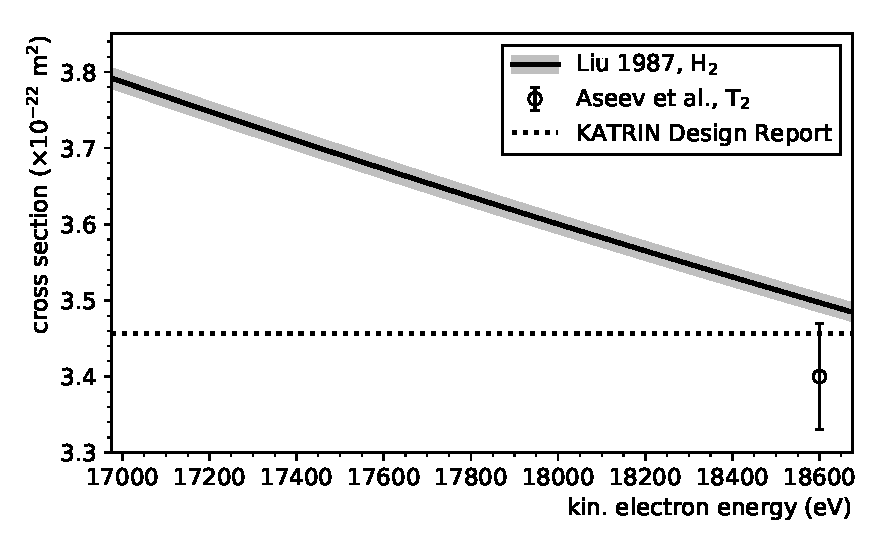
\includegraphics[width=\textwidth]{\currentFigureFolder/crossSecNoZoom.pdf}
	\xcaption{Inelastic cross section for electrons scattering off molecular hydrogen isotopologues}{Inelastic cross section for electrons scattering off molecular hydrogen isotopologues.}{The continuous line shows equation~\eqref{eq:eDepScatCrossSecSourcesCrossSecLiu} for incident electrons with non-relativistic energies with constants from equation~\eqref{eq:eDepScatCrossSecSourcesCrossSecLiuConstantsC1} and~\eqref{eq:eDepScatCrossSecSourcesCrossSecLiuConstantsC2} where the later is assumed to have an uncertainty according to equation~\eqref{eq:eDepScatCrossSecSourcesCrossSecLiuConstantsC2Uncert}. The dashed line shows equation~\eqref{eq:eDepScatCrossSecSourcesCrossSecLiuRelativistic} for incident electrons with relativistic energies. Also, the measurement by~\cite{Aseev2000} at the Troitsk neutrino mass experiment and the value stated in the KATRIN Design Report~\cite{Angrik:2005ep} are depicted. The shown energy interval is chosen according to the \gls{mtd} of the \gls{ft} measurement campaign.}
	\label{fig:eDepScatCrossSecSourcesValues}
\end{figure}

\subsection{Relation to Values of the Inelastic Scattering Cross Section in Former Works}
\label{sec:eDepScatCrossSecSourcesChoice}
As already stated and depicted in figure~\ref{fig:eDepScatCrossSecSourcesValues}, the reference cross section from the KATRIN Design Report does not match the theoretical calculations used in this thesis. Nonetheless, several former works (see subsequent section~\ref{sec:eDepScatCrossSecNuMassInf}) are based on the reference value. Comparability is of importance in the scope of this thesis (as will become apparent in section~\ref{sec:eDepScatCrossSecNuMassInf}). How this issue is addressed is explained in the following.

The cross section value stated in the KATRIN Design Report can be recovered from equation~\eqref{eq:eDepScatCrossSecSourcesCrossSecLiu} if an erroneous energy interpretation is applied. If, instead of equation~\eqref{eq:eDepScatCrossSecSourcesCrossSecNonRelEnergy}, one applies the energy interpretation
\begin{equation}
	\label{eq:eDepScatCrossSecSourcesCrossSecTDREngeryInterpretation}
	T(E) = E
	\comma
\end{equation}
the obtained cross section via equation~\eqref{eq:eDepScatCrossSecSourcesCrossSecLiu} is
\begin{equation}
\label{eq:eDepScatCrossSecSourcesTRDCrossSec}
	\sigma_\mathrm{TDR} 
	\equiv\sigma(E_\mathrm{TDR}=\SI{18565}{eV})
	=\SI{3.4559e-22}{m^2} 
	\approx\SI{3.456e-22}{m^2}
\end{equation}
as stated in the KATRIN Design Report, where the energy $E_\mathrm{TDR}$ is approximately central in the KATRIN design analysis interval (see section~\ref{sec:intSpecModelMTD}). Whether this had been the approach, that had led to the reference cross section in the KATRIN Design Report is not known. 

This work applies the energy interpretation~\eqref{eq:eDepScatCrossSecSourcesCrossSecTDREngeryInterpretation} when comparability to former works, that used the reference cross section from the KATRIN Design Report, is of importance. Otherwise, equation~\eqref{eq:eDepScatCrossSecSourcesCrossSecNonRelEnergy} is used. Corresponding indications are given on a case to case basis. The quantitative difference of these two approaches can be assessed by expanding the $\beta$-factor~\eqref{eq:eDepScatCrossSecSourcesCrossSecBetaFactor} in the ratio $E/m_\elecIndex \approx 18.575/511 \approx 0.036 \ll 1$
\begin{equation}
	\beta^2 \approx 
	2 \frac{E}{m_\elecIndex} - 
	3 \left(\frac{E}{m_\elecIndex}\right)^2
	\fullstop
\end{equation}
The energy interpretation of equation~\eqref{eq:eDepScatCrossSecSourcesCrossSecNonRelEnergy} then becomes
\begin{equation}
	T(E) \approx 0.95 \cdot E
	\comma
\end{equation}
which is a shift in energy and hence, in first order, also in the cross section of about \SI{5}{\percent} compared to the interpretation in equation~\eqref{eq:eDepScatCrossSecSourcesCrossSecTDREngeryInterpretation}. Exact calculations are given in table~\ref{tab:eDepScatCrossSecModelScatProbs}.

\section{An Energy-Dependent Scattering Model using the Poisson Distribution}
\label{sec:eDepScatCrossSecModelPoisson}
The energy-dependence of the cross section enters into the calculation of the scattering probabilities~\eqref{eq:intSpecModelNonAveragedScatProbs}. In the derivation that is given in the previous section~\ref{sec:intSpecModelResponseScattering} the dependence on the starting energy $\Esource$ of electrons is neglected. Instead, an average starting energy and hence an average scattering cross section
\begin{equation}
	\sigma_\mathrm{TDR}(E_\mathrm{TDR})=\SI{3.456e-22}{m^2}
\end{equation}  (energy interpretation as per equation~\ref{eq:eDepScatCrossSecSourcesCrossSecTDREngeryInterpretation}) is assumed. Table~\ref{tab:eDepScatCrossSecModelScatProbs} lists the corresponding scattering probabilities averaged over all starting positions and pitch angles of electrons. Additionally, the results of a Monte Carlo particle tracking simulation by~\cite{Groh2015} and the values using the energy interpretation of equation~\eqref{eq:eDepScatCrossSecSourcesCrossSecNonRelEnergy} are given. How, instead of assuming energy-independent scattering probabilities, the energy-dependence can be modeled is shown in the following.
\begin{table}[t]
	\centering
	\xcaption{Probability for severalfold electron-scattering in the \glsentryshort{wgts} - reviewed}{Probability for severalfold electron-scattering in the \glsentryshort{wgts}.}{The probabilities are averaged over all starting positions and starting pitch angles. Both, the values from a Monte Carlo (MC) particle tracking simulation and the values according to equation~\eqref{eq:intSpecModelAveragedScatProbs} are given. The  cross section was evaluated at an energy of $E_\mathrm{TDR}=\SI{18564.37463}{eV}$ for the two energy interpretations described by equation~\eqref{eq:eDepScatCrossSecSourcesCrossSecTDREngeryInterpretation} and~\eqref{eq:eDepScatCrossSecSourcesCrossSecNonRelEnergy}. Further input parameters to the calculations are a constant gas column density $\rho d = \SI{5e17}{cm^{-2}}$, 
	a \gls{wgts} length of $d=\SI{10.0820}{m}$
	and a maximum acceptance angle of $\thetaMax=\SI{50.7685}{\degree}$. The values are given with the precision needed to reproduce the results in the table below in all digits, which is the precision used in \glsentryshort{ssc}. The energy is chosen such, that $\sigma_\mathrm{TDR}=\SI{3.456000e-22}{m^2}$ is recovered in more than 3 digits as per equation~\eqref{eq:eDepScatCrossSecSourcesTRDCrossSec}.}
	\begin{tabular}{lllr}
		\toprule
		\makecell[tl]{cross section (\SI{e-22}{m^2}) $\rightarrow$} &
		3.456 &
		3.456 &
		3.673 \\
		\hline
		\makecell[tl]{source $\rightarrow$} & 
		\makecell[tl]{MC particle tracking\\ \cite{Groh2015}} & 
		\makecell[tl]{eq.~\eqref{eq:intSpecModelAveragedScatProbs} \\ \cite{Groh2015, Kleesiek2014}} &
		\makecell[tr]{eq.~\eqref{eq:intSpecModelAveragedScatProbs}}
		\\
		\hline
		\makecell[cl]{scattering count $\downarrow$} & 
		& 
	    & \\
		\hline
		\makecell{0} & $0.415 \pm 0.002$ & 0.41334 & 0.39564 \\
		\makecell{1} & $0.292 \pm 0.002$ & 0.29266 & 0.28967 \\
		\makecell{2} & $0.166 \pm 0.001$ & 0.16733 & 0.17298 \\
		\makecell{3} & $0.079 \pm 0.001$ & 0.07913 & 0.08590 \\
		\makecell{4} & $0.031 \pm 0.001$ & 0.03178 & 0.03634 \\
		\bottomrule
	\end{tabular}
	\label{tab:eDepScatCrossSecModelScatProbs}
\end{table}

\begin{figure}[th]
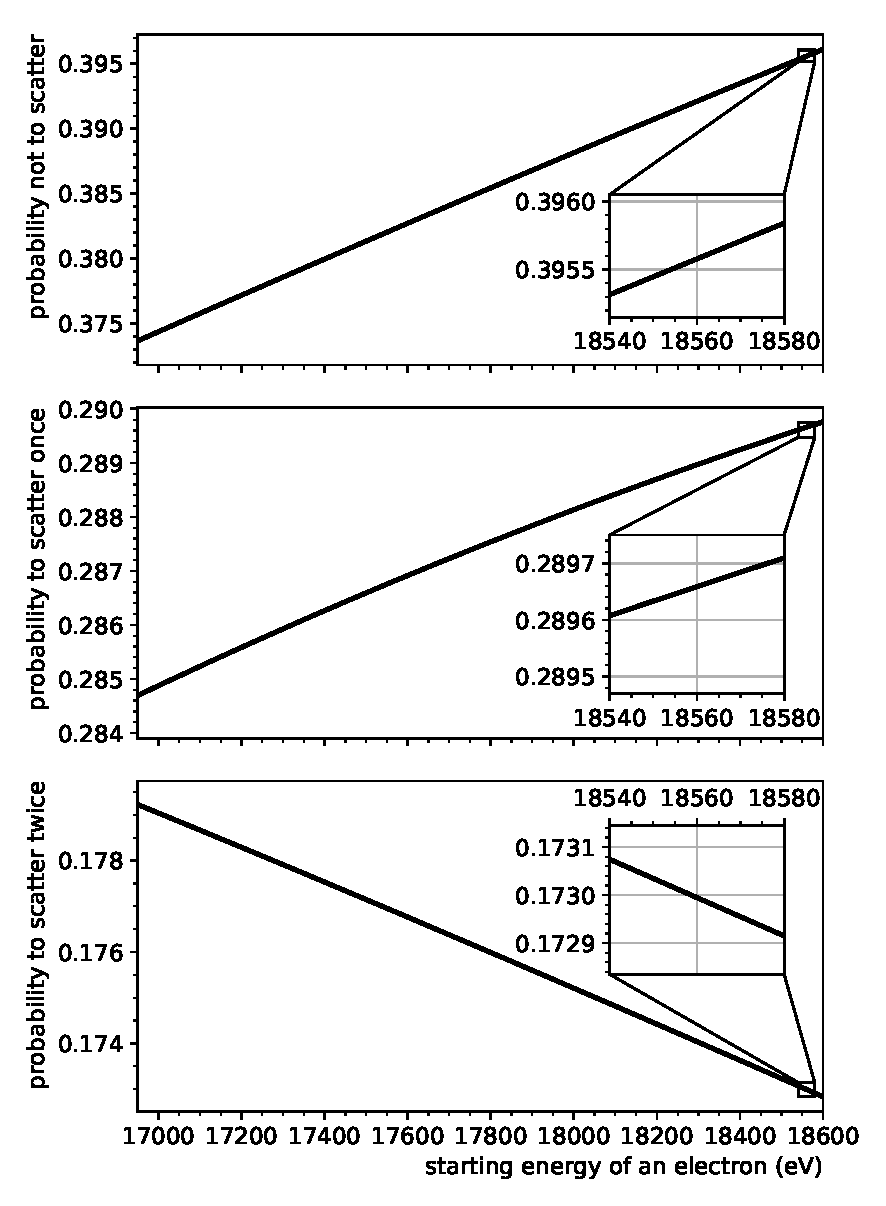
\includegraphics[width=\textwidth]{\currentFigureFolder/scatProbs012Poisson.pdf}
        \xcaption{Probability for severalfold electron-scattering in the \glsentryshort{wgts}}{Probability for severalfold electron-scattering in the \glsentryshort{wgts}.}{From top to bottom, the probability for no, one-fold and two-fold scattering are shown averaged over all starting positions and starting pitch angles of electrons in the \gls{wgts} according to the Poisson Model in equation~\eqref{eq:eDepScatCrossSecModelPoisson}. The shown energy range matches the measurement range of the \gls{ft} measurement campaign and the inset shows an energy span around the endpoint of the tritium $\upbeta$~spectrum.}
        \label{fig:eDepScatCrossSecModel}
\end{figure}

\subsection{The Poisson Model for Electron Scattering}
An expression for the probability of $l$-fold scattering of electrons within the \gls{wgts} is derived in the previous section~\ref{sec:intSpecModelResponseScattering}. The given model is independent of the energy of the electrons. Instead of using a constant cross section, the energy-dependence can be respected. The corresponding formulae from section~\ref{sec:intSpecModelResponseScattering} are repeated below, with the energy-dependence made explicit and by using an energy-dependent cross section as per equation~\eqref{eq:eDepScatCrossSecSourcesCrossSecLiu}
\begin{subequations}
\label{eq:eDepScatCrossSecModelPoisson}
\begin{align}
    \mu(\Esource,\zSource,\thetaSource) =&
    \frac{\sigma(\Esource)}{\cos\thetaSource}
    \int_{\zSource}^{d/2} \rho(z)\d z \label{eq:energydepScatProbsPoissonExpectedScatCount} 
    \comma\\
    P_l(\Esource,\zSource,\thetaSource) =&
    \mathrm{Poisson}(\mu(\Esource,\zSource,\thetaSource),l) \label{eq:eDepScatCrossSecModelPoissonNonAveragedScatProbs} 
    \comma \\
    \bar{P}_l(\Esource) =&
    \frac{1}{d \cdot (1-\cos(\thetaMax))} 
      \int_{-d/2}^{d/2}  
          \int_{0}^{\theta_{max}} 
            \sin(\thetaSource)
            \mathrm{Poisson}(\mu(\Esource,\zSource,\thetaSource),l)
          \d\thetaSource
      \d\zSource
      \label{eq:eDepScatCrossSecModelPoissonAveragedScatProbs}
    \fullstop
\end{align}
\end{subequations}
As a reminder, $\bar{P}_l(\Esource)$ in equation~\eqref{eq:eDepScatCrossSecModelPoissonAveragedScatProbs} denotes the probability for $l$-fold scattering of an electron with a starting kinetic energy $\Esource$ averaged over all starting positions and pitch angles in the \gls{wgts}. In the following, this model is denoted ``Poisson model''. 

\subsection{Properties of the Poisson Model for Electron Scattering}
\label{sec:eDepScatCrossSecModelPoissonProperties}
Figure~\ref{fig:eDepScatCrossSecModel} shows the Poisson model as per equation~\eqref{eq:eDepScatCrossSecModelPoisson}. Table \ref{tab:eDepScatCrossSecModelScatProbs} lists the scattering probabilities for an energy-independent Poisson model (see section~\ref{sec:intSpecModelResponseScattering}) and a reference cross section $\sigma(E\approx\SI{18564}{eV})=\SI{3.673e-22}{m}$. The energy-dependent Poisson model recovers the energy-independent model exactly at the corresponding energy as expected.

\paragraph{Trend of the Energy-Dependence}
\begin{figure}[th]
	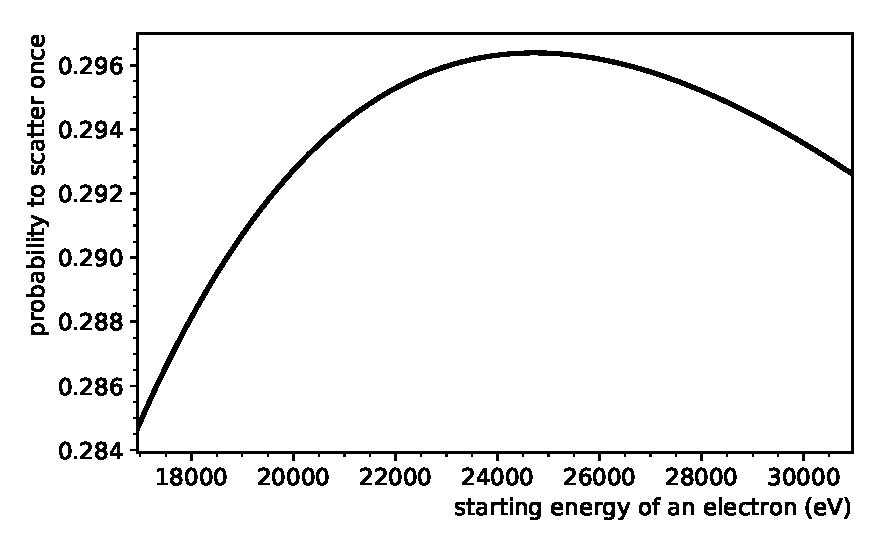
\includegraphics[width=\textwidth]{\currentFigureFolder/scatProbs1Poisson_extendedEnergyRange.pdf}
	\xcaption{Probability for one-fold electron-scattering in the \glsentryshort{wgts} in an extended energy range}{Probability for one-fold electron-scattering in the \glsentryshort{wgts} in an extended energy range.}{The graph shows the probability of one-fold scattering according to equation~\eqref{eq:eDepScatCrossSecModelPoissonAveragedScatProbs}. It emphasizes the change of sign in the derivative at approximately \SI{24.7}{keV}.}
	\label{fig:eDepScatCrossSecModelPoissonP1ExtendedEnergyRange}
\end{figure}
As depicted in figure~\ref{fig:eDepScatCrossSecModel}, for an increasing starting energy of electrons within the \gls{wgts}, the probability for no and one-fold scattering also increases, while the probability for two-fold scattering decreases. This paragraph aims to give an intuitive argument for this change of sign in the derivative $\d \bar{P}_l(\Esource) / \d \Esource$ in the transition from $l=1$ to $l=2$. The Poisson model $\bar{P}_l(\Esource)$ is a probability density in $l$ for a fixed $\Esource$ (see appendix~\ref{sec:appendixEDepScatCrossSecPoissonModelProbDensityProof} for a proof). Hence, the expected scattering count for an energy within the range of starting energies $\Esource \in [\SI{17}{keV}, \SI{18.6}{keV}]$, that is depicted in figure~\ref{fig:eDepScatCrossSecModel}, can be calculated (numerically)
\begin{equation}
\label{eq:eDepScatCrossSecModelPoissonExpectedScatCount}
\begin{split}	
	\bar{l}(\SI{17.0}{keV}) &= 
	\sum_{l}^{\infty} \bar{P}_l(\SI{17.0}{keV}) \cdot l \approx 1.23 \\	
	\bar{l}(\SI{18.6}{keV}) &= 
	\sum_{l}^{\infty} \bar{P}_l(\SI{18.6}{keV}) \cdot l \approx 1.14
	\fullstop
\end{split}
\end{equation} 
In other words, electrons with a starting energy between \SI{17}{keV} and \SI{18.6}{keV} are expected to scatter between 1 and 2 times on their way through the \gls{wgts} (averaged over all starting positions and pitch angles). Then, the illustrative line of argument is the following: 
\begin{align*}
	&\text{ the starting energy $\Esource$ increases} \\ \Rightarrow
	&\text{ the scattering cross section decreases (see figure~\ref{fig:eDepScatCrossSecSourcesValues})} \\ \Rightarrow
	&\text{ scattering becomes less likely} \\ \Rightarrow
	&\text{ $\bar{l}$ decreases and moves closer to 1 and away from 2} \\ \Rightarrow
	&\text{ the probability for no and one-fold scattering increases,} \\
	&\text{ while the probability for more than one scattering decreases}
	\fullstop
\end{align*} 
This is in accordance with the trend of the energy-dependence depicted in figure~\ref{fig:eDepScatCrossSecModel}. Also, if this reasoning is correct, the sign of $\d \bar{P}_1(\Esource) / \d \Esource$ for one-fold scattering should change for sufficiently high energies and the probability to scatter once should decrease. This is indeed the case as depicted in figure~\ref{fig:eDepScatCrossSecModelPoissonP1ExtendedEnergyRange}. The decrease starts at an energy of roughly \SI{24.7}{keV}. This might for example be of relevance for the measurement of Krypton conversion lines in calibration measurements because the corresponding electron energies are above \SI{30}{keV}~\cite{venos2018}.


\paragraph{Limit of the Poisson Model for Electron Scattering}
The Poisson model is exact for the probability of no scattering $\bar{P}_0(\Esource)$, but it does not hold for one or more scatterings because an electron loses energy when scattering. The scattering cross section increases with decreasing energy (see figure~\ref{fig:eDepScatCrossSecSourcesValues}) and the electron becomes more likely to scatter again. In other words, the probabilities of individual scattering processes are no longer independent when respecting the dependence on the electron energy. This violates one of the preconditions to model the scattering probabilities via a Poisson distribution. Another model beyond the description via a Poisson distribution is suggested in the subsequent section~\ref{sec:eDepScatCrossSecModelExtended}. However, at the current stage, this extended model poses computational difficulties as is discussed in section~\ref{sec:eDepScatCrossSecExtendedModelNumEval}. The aim of this thesis is the assessment of energy-dependent effects. This can already be achieved with the Poisson model as shown in the previous paragraphs. Therefore, the Poisson model was further used to address the energy-dependent effects in the scope of neutrino mass inference.
\FloatBarrier

\paragraph{Implementation and Performance}
Within the scope of this thesis, the energy-dependent Poisson model of equation~\eqref{eq:eDepScatCrossSecModelPoisson} was implemented into the \gls{ssc} software framework. The energy-dependence of the scattering cross section may not be negligible in neutrino mass inference as is explained in the subsequent section~\ref{sec:eDepScatCrossSecNuMassInf}. For that reason, the impact on the fitting run time by using an energy-dependent cross section was probed. Depending on the \gls{mtd}, a fit might become slower by a factor of 40 to 120. This is due to the fact, that, when integrating over the energy loss in the response function in equation~\eqref{eq:intSpecModelResponse}, the scattering probabilities have to be recomputed in every step of the numerical integration. It might be beneficial to investigate whether the evaluation can be speed up in the future. For example, it might be sufficient to only compute the energy-dependent scattering probabilities for a limited set of energies and interpolate them in-between those energies.

\section{Effects of Systematic Cross-Section Offsets in Neutrino Mass Inference}
\label{sec:eDepScatCrossSecNuMassInf}
It was investigated, how much the squared neutrino mass that is inferred from a KATRIN measurement would be shifted if the energy-dependence of the scattering cross section is neglected in the corresponding fitting procedure. The comparability to former results is of importance within this section. For that reason, the energy interpretation of equation~\eqref{eq:eDepScatCrossSecSourcesCrossSecTDREngeryInterpretation} is used, which yields a cross section of $\sigma_\mathrm{TDR}=\SI{3.456e-22}{m^2}$ at an energy of \SI{18565}{eV} within the KATRIN design analysis interval. There are several previous works that studied similar effects~\cite{Antoni2015,Groh2015,SeitzM2019,Kuckert2016,Kuckert2018}. In section~\ref{sec:eDepScatCrossSecNuMassInfGroh}, the results from~\cite{Groh2015} are reviewed representatively for the mentioned works because they might intuitively contradict the results obtained in this thesis. In section~\ref{sec:eDepScatCrossSecNuMassInfThisWork}, the results of this thesis are listed. And in section~\ref{sec:eDepScatCrossSecNuMassInfRelateGrohAndFormerWork}, an argument is given, why both sets of results are assumed to be in accordance.

\subsection{Neutrino Mass Shifts for an Energy-Independent Cross-Section Offset from Former Works}
\label{sec:eDepScatCrossSecNuMassInfGroh}
In~\cite{Groh2015}, it was investigated how much a constant offset of the cross section would shift the inferred squared neutrino mass if the offset were neglected in the analysis. A rule of thumb for the shift in dependence on the relative offset of the cross section $\Delta\sigma/\sigma_\mathrm{TDR}$ is given~\cite{Groh2015}
\begin{equation}
	\label{eq:eDepScatCrossSecNuMassInfShiftRuleOfThumb}
	\frac{\Delta\nuMass^2(\Delta\sigma)}{\SI{e-3}{eV^2}} =
	-0.45
	-1204\cdot
	\frac{
		\Delta\sigma
	}{
		\sigma_\mathrm{TDR}
	}
	\qquad \text{ with } \quad 
	\sigma_\mathrm{TDR} = \SI{3.456e-22}{m^{-2}}
	\fullstop
\end{equation}
This rule of thumb was deduced via a linear approximation of several neutrino mass shifts in dependence of the relative cross section offset. Although, it can only be used for rough estimations, it serves well for the discussion in the following sections. Using the energy interpretation of the KATRIN Design Report (eq.~\ref{eq:eDepScatCrossSecSourcesCrossSecTDREngeryInterpretation}) and the numerical inversion of the cross section formula (eq.~\ref{eq:eDepScatCrossSecSourcesCrossSecLiu}), in the KATRIN design analysis interval of \SI{30}{eV}, the relative offset of the cross section caused by the energy-dependence is
\begin{equation}
	\label{eq:eDepScatCrossSecNuMassInfRelativeCrossSecOffset}
	\left|
	\frac{
		\Delta\sigma
	}{
		\sigma_\mathrm{TDR}
	}
	\right| < \SI{0.1}{\percent}
	\fullstop
\end{equation}
Thus, the rule of thumb~\eqref{eq:eDepScatCrossSecNuMassInfShiftRuleOfThumb} yields
\begin{equation}
	\label{eq:eDepScatCrossSecNuMassInfShiftEstimate}
	\left|
		\Delta\nuMass^2(\Delta\sigma)
	\right| < \SI{2e-3}{eV^2} 
\end{equation}
within the KATRIN design analysis interval of \SI{30}{eV}.

\subsection{Neutrino Mass Shifts for an Energy-Dependent Cross-Section Offset}
\label{sec:eDepScatCrossSecNuMassInfThisWork}
\begin{figure}[t]
	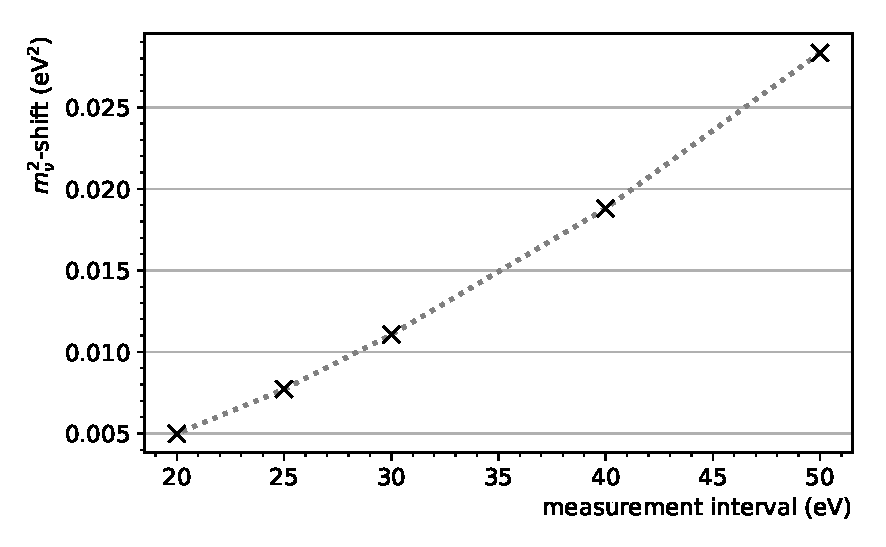
\includegraphics[width=\textwidth]{\currentFigureFolder/nuMassShiftForEDepCrossSec.pdf}
	\xcaption{Shift of an inferred squared neutrino mass induced by a neglected energy-dependence of the inelastic scattering cross section}{Shift of an inferred squared neutrino mass induced by a neglected energy-dependence of the inelastic scattering cross section.}{The neutrino mass was inferred from data that was simulated using an energy-dependent inelastic scattering cross section as per equation~\eqref{eq:eDepScatCrossSecSourcesCrossSecLiu} (with an energy interpretation according to equation~\eqref{eq:eDepScatCrossSecSourcesCrossSecTDREngeryInterpretation} for compatibility with the KATRIN Design Report) and using a nominal four-parameter fit model that assumes a constant cross section of $\sigma_\mathrm{TDR}=\SI{3.456e-22}{m^2}$. The procedure was repeated for five different measurement intervals (respectively \gls{mtd}s) $[E_0-\alpha, E_0+\SI{5}{eV}]$ based on the KATRIN Design Report where $\alpha$ is denoted on the abscissa and $E_0=\SI{18575}{eV}$ is the endpoint of the $\upbeta$ spectrum. The \gls{mtd}s are listed in appendix~\ref{sec:appendixEDepScatCrossSecMTDs}. The markers show the results for the obtained shift of the squared neutrino mass and the dotted line is an interpolation in-between. The study was done once with a free fit parameter for the endpoint and once having it fixed to the simulation truth in order to show the influence on the sign of the shift of the squared neutrino mass (for details refer to the the main text).}
	\label{fig:eDepScatCrossSecNuMassInfShifts}
\end{figure}
In the scope of this thesis, an energy-dependent offset of the cross section was investigated (in contrast to a constant one in~\cite{Groh2015}). A KATRIN neutrino mass measurement for a neutrino mass of \SI{0}{eV} was simulated using an energy-dependent cross section\footnote{In all studies presented in this chapter, the simulated electron detector counts were substituted by their expectation values as opposed to fluctuated according to Poissonian statistics. In other words, no ensemble testing was done. For more details on such an Asimov data set and why it can reasonably be assumed to be representative for an ensemble, see section~\ref{sec:katrinElossStatisticsAsimov}.}. A model that uses a constant cross section was fitted to the simulated spectrum. This procedure was repeated for five different \gls{mtd}s of different measurement intervals. Figure~\ref{fig:eDepScatCrossSecNuMassInfShifts} shows the results. For the KATRIN design measurement interval of~\SI{30}{eV}, the difference from \SI{0}{eV}, respectively the shift of the squared neutrino mass, is
\begin{equation}
	\label{eq:eDepScatCrossSecNuMassInfShiftByThisThesis}
	\Delta\nuMass^2 = \SI{1.09e-2}{eV^2}
	\fullstop
\end{equation}
First, it should be noted that this value is greater by a factor of $\sim5$ than the one stated above in equation~\eqref{eq:eDepScatCrossSecNuMassInfShiftEstimate}, that was estimated using the results from~\cite{Groh2015}. This issue is addressed in the subsequent section~\ref{sec:eDepScatCrossSecNuMassInfRelateGrohAndFormerWork}. Further aspects are discussed in the following paragraph:

\paragraph{Sign of the Shift of the Squared Neutrino Mass}
Using an energy-dependent cross section in the simulation and neglecting it in neutrino mass inference yields a higher $\upbeta$ electron count in the endpoint region than expected (see figure~\ref{fig:eDepScatCrossSecNuMassInfIntegralRate}) because the cross section decreases with higher energies and electrons of higher energies are less probable to scatter. On one hand, a higher $\upbeta$ electron count for energies in the endpoint region of the $\upbeta$ spectrum can be caused by a lower squared neutrino mass. On the other hand, a higher $\upbeta$ electron count can also be caused by a higher endpoint of the $\upbeta$ spectrum. These two effects counterbalance each other, which makes it difficult to make an intuitive, qualitative statement about the sign of the shift of the squared neutrino mass. As shown in equation~\eqref{eq:eDepScatCrossSecNuMassInfShiftByThisThesis}, the shift of the squared neutrino mass is positive. However, if the above reasoning is correct, then one should obtain a flip in the sign of the shift if the endpoint is not taken as a free fit parameter, but fixed to the simulation truth. Figure~\ref{fig:eDepScatCrossSecNuMassInfShifts} shows that this is indeed the case.

\paragraph{Significance for the KATRIN Experiment}
The shift of the squared neutrino mass in equation~\eqref{eq:eDepScatCrossSecNuMassInfShiftByThisThesis} takes a sizable fraction of the systematic budget of \SI{1.7e-2}{eV^2} (see eq.~\ref{eq:statMethodsSensitivtyFromEnsembleTDRSysBudget}) of the KATRIN experiment, but is still smaller. Hence, whether the effect of the energy-dependence of the scattering cross section can be neglected depends on the contribution of other systematic effects and can not yet fully be assessed (see for example~\cite{SeitzM2019} for a comprehensive list of systematic effects with regard to the KATRIN experiment).

It should be mentioned that KATRIN's design allows to measure the product of the gas column density and the inelastic scattering cross section $\rho d \cdot \sigma(E)$ for a fixed electron energy~$E$ using the electron gun. In order to respect the energy dependence of the cross section, it is necessary to incorporate a corresponding model, such as the formula for the energy-dependent cross section (eq.~\ref{eq:eDepScatCrossSecSourcesCrossSecLiu}). This might enable the measurement of the two constants $C_1$ and $C_2$ in said formula. Therefore, $\rho d \cdot \sigma(E)$ has to be measured for multiple energies $E$. Such measurements were already conducted at the KATRIN experiment. However, results that respect the energy-dependence of the scattering cross section are not yet available at the time of writing this thesis.

\subsection{Relation of the Shifts for an Energy-Dependent and -Independent Cross-Section Offset}
\label{sec:eDepScatCrossSecNuMassInfRelateGrohAndFormerWork}
In the scope of this thesis, the shift of an inferred neutrino mass that is introduced by neglecting the energy-dependence of the cross section was investigated. Former works investigated the shift when neglecting a constant offset of the cross section. The shift obtained in this thesis in equation~\eqref{eq:eDepScatCrossSecNuMassInfShiftByThisThesis} is $\sim5$ times larger than the one obtained by the former study in~\cite{Groh2015} under equation~\eqref{eq:eDepScatCrossSecNuMassInfShiftEstimate}, although the energy-dependent offset of the cross section is never greater than the constant offset investigated by~\cite{Groh2015}. This might be contra intuitive, but a possible explanation is the following: The fit parameter for the signal amplitude $\sigAmp$ in a nominal KATRIN fit (see section~\ref{sec:statMethodsStandardFit}) can partly compensate for a constant offset of the cross section. However, it cannot compensate for an energy-dependent one equally well. This is demonstrated below:

The study from~\cite{Groh2015} was reproduced with a free fit parameter for the signal amplitude $\sigAmp$. The reproduced study was in accordance with the values in~\cite{Groh2015}. Then, $\sigAmp=1$ was fixed. The results are shown in figure~\ref{fig:eDepScatCrossSecNuMassInfShiftsForConstCrossSec}. A relative cross section offset of $
\left|
	\Delta\sigma/\sigma_\mathrm{TDR}
\right| \approx \SI{0.1}{\percent}
$ (see equation~\ref{eq:eDepScatCrossSecNuMassInfRelativeCrossSecOffset}) yields a shift of the squared neutrino mass, that is larger by almost an order of magnitude with a fixed $\sigAmp$ as opposed to leaving $\sigAmp$ as a free parameter. The shift is then greater than the one obtained in the the study presented in the previous section~\ref{sec:eDepScatCrossSecNuMassInfThisWork} that uses an energy-dependent cross section in the \SI{30}{eV} measurement interval. This verifies, that the fit parameter for the signal amplitude $\sigAmp$ can partly compensate for a constant offset of the cross section. 

Additionally, the following plausibility argument can be given: Figure~\ref{fig:eDepScatCrossSecNuMassInfIntegralRate} shows the simulated integral rate for different cross section models normalized to the integral rate obtained by using the model with a constant cross section $\sigma_\mathrm{TDR}$ from the KATRIN Design Report. The integral rates that are based on a model with a constant, energy-independent cross section differ from each other by almost a constant factor (variations $<2\times10^{-4}$). This implies, when one of these models is used in a simulation of a KATRIN measurement and another model is used in a corresponding fit for neutrino mass inference, their difference can be compensated by the fit parameter for the signal amplitude $\sigAmp$. However, the model that uses an energy-dependent cross section does not differs from the one with the constant cross section $\sigma_\mathrm{TDR}$ by a factor, that varies over the energy range. Such a difference can not be compensated by the fit parameter for the signal amplitude $\sigAmp$.

\begin{figure}[t]
	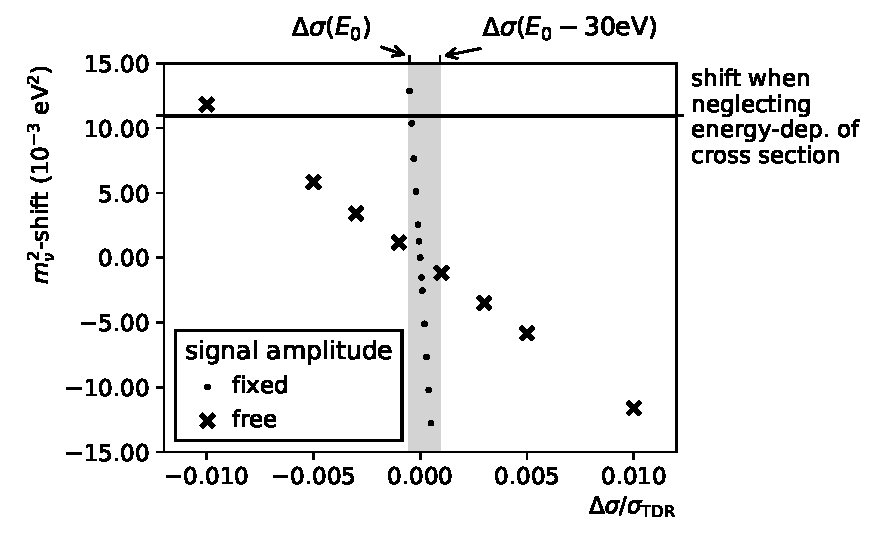
\includegraphics[width=\textwidth]{\currentFigureFolder/nuMassShiftForConstCrossSec.pdf}
	\xcaption{Shift of an inferred squared neutrino mass induced by a neglected constant offset of the inelastic scattering cross section}{Shift of an inferred squared neutrino mass induced by a neglected constant offset of the inelastic scattering cross section.}{The neutrino mass was inferred from data that was simulated using different constant inelastic scattering cross sections. The abscissa shows the offset of the used inelastic scattering cross section relative to $\sigma_\mathrm{TDR}=\SI{3.456e-22}{m^2}$, which was used in the assumed fit model. In an energy-dependent scenario, a cross section corresponds an energy of incident electrons as per equation~\eqref{eq:eDepScatCrossSecSourcesCrossSecLiu}. The cross section range, that corresponds the design KATRIN analysis energy interval of \SI{30}{eV} is depicted as a gray band (energy interpretation as per eq.~\ref{eq:eDepScatCrossSecSourcesCrossSecTDREngeryInterpretation}). The analysis was done twice: once with a free parameter for the signal amplitude, which reproduced the results given in~\cite{Groh2015}~(figure 6.31 on page 221); the second analysis had this parameter fixed. The shift  obtained for $\Delta\sigma/\sigma_\mathrm{TDR}\approx\SI{-0.1}{\percent}$ and a fixed signal amplitude is greater than the shift obtained when neglecting the energy-dependence of the cross section within the \SI{30}{eV} measurement interval (depicted by the horizontal line).}
	\label{fig:eDepScatCrossSecNuMassInfShiftsForConstCrossSec}
\end{figure}


\begin{figure}[t]
	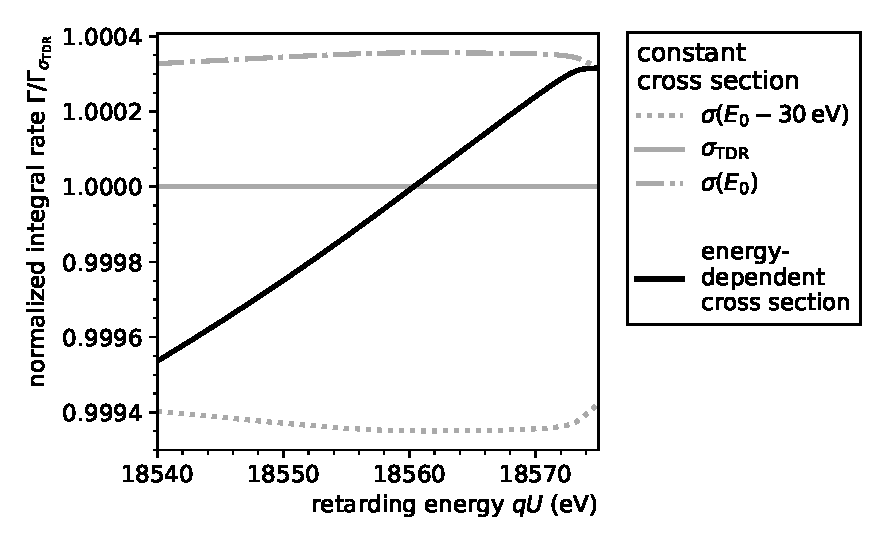
\includegraphics[width=\textwidth]{\currentFigureFolder/normedIntegralRate.pdf}
	\xcaption{Simulated integral $\upbeta$-electron rate using different models of the cross section for inelastic electron-scattering}{Simulated integral $\boldsymbol{\upbeta}$-electron rate using different models of the cross section for inelastic electron-scattering.}{The abscissa shows the energy range of the design KATRIN analysis interval of \SI{30}{eV}. The lines show the integral rate of $\upbeta$~electrons for different models for the inelastic scattering cross section normalized to the model that uses the constant cross section $\sigma_\mathrm{TDR}=\SI{3.456e-22}{m^2}$. The gray lines use a model with a constant cross section. The cross section values can be identified with electron energies as per equation~\eqref{eq:eDepScatCrossSecSourcesCrossSecLiu} and the energy interpretation of equation~\eqref{eq:eDepScatCrossSecSourcesCrossSecTDREngeryInterpretation} with $\sigma(E_0-\SI{30}{eV}=\SI{18545}{eV})=\SI{3.459e-22}{m^2}$ and $\sigma(E_0=\SI{18575}{eV})=\SI{3.454e-22}{m^2}$. The black line shows the simulated integral rate for an energy-dependent cross section. This graph emphasizes that the integral rates for models using a constant cross section differ by an almost constant factor, whereas the rate using an energy-dependent cross section differs from the others by a varying factor.}
	\label{fig:eDepScatCrossSecNuMassInfIntegralRate}
\end{figure}
\FloatBarrier

\section{An Energy-Dependent Scattering Model beyond Using the Poisson Distribution}
\label{sec:eDepScatCrossSecModelExtended}
In the previous section~\ref{sec:eDepScatCrossSecModelPoisson} the scattering probabilities are modeled using a Poisson distribution. This introduces an error for the following reason: A scattering electron loses energy. The scattering cross section increases with decreasing energy (see figure~\ref{fig:eDepScatCrossSecSourcesValues}) and the electron becomes more likely to scatter again. In other words, the probabilities of individual scattering processes are not independent when respecting the dependence on the electron energy. This violates one of the preconditions to model the scattering probabilities via a Poisson distribution. 

This section aims to quantify the error that is introduced by the approximate modeling via a Poisson distribution. Another model is suggested\footnote{The idea was inspired by a model in~\cite{Groh2015} that incorporates changes of the electron pitch angle due to scattering.} in section~\ref{sec:eDepScatCrossSecExtendedModelFormalism} that partly accounts for the energy loss of electrons in the formalism of the scattering probabilities. The suggested model was evaluated numerically as it includes one limit and two integrals that could not yet be solved analytically. The numerical accuracy had to be good enough to decide whether it differs significantly from the Poisson model or not. At the same time, a balance between the numerical accuracy and the evaluation run time had to be found. This matter is described in detail in section~\ref{sec:eDepScatCrossSecExtendedModelNumEval}. The results of the numerical evaluation are discussed in section~\ref{sec:eDepScatCrossSecExtendedModelDiscussion}.

\subsection{Mathematical Formalism of the Extended Model for Electron Scattering}
\label{sec:eDepScatCrossSecExtendedModelFormalism}
In the following, a model for the probability of electron-scattering in the \gls{wgts} that depends on the electron energy is derived. The difficulty lies in the fact, that an electron that scatters loses energy and hence its probability to scatter a second time is different from the first time. The presented model assumes the same fixed energy loss $\epsilon$ for each scattering in contrast to a realistic distribution as given by the energy loss function (see figure~\ref{fig:intSpecModelAseevEloss}). This was sufficient to show a difference in the Poisson model and the model suggested below. However, a more accurate description would incorporate the full energy loss function. This may be the subject of a future study. 

The aim of this section is the derivation of an expression $\bar{P}^{\star}_l(\Esource)$ that denotes the probability of $l$-fold scattering for an electron with a starting energy $\Esource$ averaged over all starting positions and pitch angles assuming a fixed energy loss $\epsilon$ per scattering.

The expected amount of scatterings for an electron when traveling through the whole \gls{wgts} volume of length $d$ filled with a gas of constant density $\rho$ is (see equation~\ref{eq:intSpecModelExpectedScatteringCount})
\begin{equation}
\label{eq:eDepScatCrossSecExtendedModelFormalismExpectedScatCount}
\mu(E,\thetaSource) =
\frac{\sigma(E)\rho d}{\cos\thetaSource},
\end{equation}
where $E$ denotes the electron's kinetic energy; $\thetaSource$ the starting pitch angle; and $\sigma(E)$ the energy dependent scattering cross section. It should be noted that the energy $E$ is denoted without and index S here, because, in the following, this formula is reused for different electron energies, not only the starting energy of an electron.

In the following, the volume of the \gls{wgts} is thought of being divided into $N$ slices of equal width $w=L/N$ (and later the limit $N\rightarrow\infty$ is applied). $N$ is chosen sufficiently large that the probability for an electron to scatter twice within one slice is essentially zero. Then, for large $N$, the probability to scatter within one slice is $\mu(E,\thetaSource)/N$. The probability not to scatter within $n \leq N$ slices is
\begin{equation}
p_0(E,\thetaSource,n) =
\left(
1-\frac{\mu(E,\thetaSource)}{N}
\right)^n
\fullstop
\end{equation}
Let ``Poisson($\mu$,$l$)'' denote the Poisson distribution with expectation value $\mu$ and evaluated at $l$. Using the well known limit for the Euler constant, one obtains for $n=N$ and $N\rightarrow\infty$ that $p_0$ is a Poisson distribution with the expectation value $\mu$ from equation~\eqref{eq:eDepScatCrossSecExtendedModelFormalismExpectedScatCount} and evaluated at $l=0$ 
\begin{align}
\label{eq:eDepScatCrossSecExtendedModelFormalismRecoveryOfPoisson}
\lim_{N\rightarrow\infty} 
p_0(E,\thetaSource,N) =
\lim_{N\rightarrow\infty} 
\left(
1-\frac{\mu(E,\thetaSource)}{N}
\right)^N =
\mathrm{e}^{-\mu(E,\thetaSource)} = 
\mathrm{Poisson}(\mu(E,\thetaSource), 0)
\fullstop
\end{align}
In other words, for no scattering, the Poisson model for the scattering probabilities as described in section~\ref{sec:eDepScatCrossSecModelPoisson} is recovered.

Assuming a constant energy loss $\epsilon$ per scattering, the probability to scatter $l>0$ times within $n<N$ slices can be expressed recursively
\begin{equation}
\label{eq:eDepScatCrossSecExtendedModelFormalismCore}
p_l(E,\thetaSource,n) =
\underbrace{
	\sum_{k=l}^{n}
}_{(4)}
\underbrace{
	p_{l-1}(E,\thetaSource,k-1)
	\vphantom{\sum_{k=l}^{n}}
}_{(1)}
\underbrace{
	\left(
	1-p_0(E-(l-1)\epsilon,\thetaSource,1)
	\right)
	\vphantom{\sum_{k=l}^{n}}
}_{(2)}
\underbrace{
	p_0(E-l\epsilon,\thetaSource,n-k)
	\vphantom{\sum_{k=l}^{n}}
}_{(3)}
\fullstop
\end{equation}
The idea behind this expression is the following: One imagines an electron with an energy $E$ that travels through $n$ \gls{wgts} slices, scatters $l$ times in total and the last time in the $k$th slice. Hence, it must have scattered $l-1$ times in the $k-1$ slices before the $k$th slice and must not scatter in the $n-k$ slices to follow. In that regard, the above expressions have the following meaning:
\begin{enumerate}[(1)]
	\item Probability to scatter $l-1$ times within $k-1$ slices with a kinetic energy of $E$.
	\item Probability to scatter once within the $k$th slice with a kinetic energy of $E-(l-1)\epsilon$.
	\item Probability not to scatter within the remaining $n-k$ slices with a kinetic energy of $E-l\epsilon$.
	\item Sum over all slices $k$ where the electron could scatter the last time. The sum starts at $l$ (as opposed to 1) because the probability to scatter $l-1$ times within less than $k=l-1$ slices (term (1)) is 0 due to the made assumption, that in the limit of a large amount of slices $N$ an electron does not scatter twice within one slice.
\end{enumerate}
The probability to scatter $l$ times can be averaged over all starting positions of electrons respectively starting slices. In this regard, $\nSource$ denotes the amount of slices an electron has to pass through depending on its starting slice (including its starting slice). Then the average is
\begin{equation}
\label{eq:eDepScatCrossSecExtendedModelFormalismZAverage}
\bar{p}_l(E,\thetaSource) = 
\frac{1}{N}
\sum_{\nSource=1}^{N} p_l(E,\thetaSource,\nSource) \approx
\frac{1}{d}
\int_{0}^{d}
p_l(E,\thetaSource,
\left\lceil N \frac{\zSource}{d}\right\rceil
)
\d \zSource
\fullstop
\end{equation}
Here, the averaging sum is approximated by an integral as this helps cutting down on run time in a numerical evaluation. This is due to the fact, that in a numerical evaluation a large number $N$ ($\sim10^5$) of slices has to be chosen and the sum would have many terms. However, a numerical integration can achieve an accurate result with a smaller set of supporting points (see subsequent section~\ref{sec:eDepScatCrossSecExtendedModelNumEval}). 

Then, the limit $N\rightarrow\infty$ can be applied
\begin{equation}
P^{\star}_l(\Esource,\thetaSource) = 
\lim_{N\rightarrow\infty} \bar{p}_l(\Esource,\thetaSource)
\fullstop
\label{eq:eDepScatCrossSecExtendedModelFormalismPitchAngleDepScatProbs}
\end{equation}
$P^{\star}_l(\Esource,\thetaSource)$ denotes the probability for an electron to scatter $l$ times when traveling through the whole \gls{wgts} with a starting energy $\Esource$ and pitch angle $\thetaSource$ averaged over all starting positions. Finally, this expression can be averaged over all starting pitch angles in order to obtain the energy dependent scattering probabilities
\begin{equation}
\bar{P}^{\star}_l(\Esource) = 
\frac{1}{1-\cos\thetaMax}
\int_0^{\thetaMax}
\sin \thetaSource
P^{\star}_l(\Esource,\thetaSource) 
\d \thetaSource
\fullstop
\label{eq:eDepScatCrossSecExtendedModelFormalismAveragedDepScatProbs}
\end{equation}
$\bar{P}^{\star}_l(\Esource)$ denotes the probability for $l$-fold scattering of an electron with a starting energy $\Esource$ averaged over all starting positions and pitch angles assuming a fixed energy loss $\epsilon$ per scattering. In the following, this model is called the ``extended model''.

\subsection{Numerical Accuracy and Cross-Check of the Extended Model for Electron Scattering}
\label{sec:eDepScatCrossSecExtendedModelNumEval}
\begin{figure}[t]
	\centering
	\includegraphics{chapter/energyDependentCrossSec/fig/scatProb1_numericalAccuracy.pdf}
	\xcaption{Accuracy of the numerical evaluation of the extended model of the probability for electron-scattering in the \glsentryshort{wgts}}{Accuracy of the numerical evaluation of the extended model of the probability for electron-scattering in the \glsentryshort{wgts}.}{The extended model is given by equation~\eqref{eq:eDepScatCrossSecExtendedModelFormalismAveragedDepScatProbs} and the Poisson model is given by equation~\eqref{eq:eDepScatCrossSecModelPoisson}. For both models, the energy of the incident electrons was taken such that the Poisson model yields the values already given in table~\ref{tab:eDepScatCrossSecModelScatProbs}. The left column shows the dependence on the number $N$ of slices of the \gls{wgts}. The right column shows the dependence on the order of Gaussian quadrature that was used to evaluate the two integrals in the extended model. The Poisson model is independent of these features and can be evaluated exactly (limited by machine number precision). In the left column, the order of Gaussian quadrature was fixed to 5 and in the right column, the number of slices was fixed to $5\times10^{5}$. The upper row shows the numerical evaluation of the extended model for no energy loss per scattering (markers). Its exact solution is given by the Poisson model (line). The lower row shows the extended model for an energy loss of \SI{12.6}{eV} per scattering. The upper row shows that the numerical evaluation of the extended model is within a distance of less than $3\times10^{-6}$ of its exact solution and the lower row shows convergence on the $10^{-5}$ level. These results make it plausible to assume a numerical accuracy on the $10^{-5}$ level or better for the shown configurations of the numerical evaluation of the extended model.}
	\label{fig:eDepScatCrossSecExtendedModelNumEval}
\end{figure}
For the evaluation of the energy-dependent scattering probabilities according to the extended model in equation~\eqref{eq:eDepScatCrossSecExtendedModelFormalismAveragedDepScatProbs} the fixed energy loss $\epsilon=\SI{12.6}{eV}$ per scattering was chosen as it is the most probable energy loss for electrons traveling through tritium gas (see figure~\ref{fig:intSpecModelAseevEloss}). The mean value would also have been a possible choice. But the energy loss function as depicted in figure~\ref{fig:intSpecModelAseevEloss} is not normalized to $[0, \infty)$, which poses the problem of finding a suitable energy interval, with respect to which the mean value is calculated. In other words, at the current stage, a certain arbitrarity concerning the energy loss per scattering could not be avoided. As already mentioned, a future study might consider a more comprehensive incorporation of the energy loss function.

The extended model in equation~\eqref{eq:eDepScatCrossSecExtendedModelFormalismAveragedDepScatProbs} was evaluated numerically:
\begin{itemize}
	\item Taking the limit~$N\rightarrow\infty$ in equation~\eqref{eq:eDepScatCrossSecExtendedModelFormalismPitchAngleDepScatProbs} was replaced by choosing a large $N$.
	\item The averaging integral over the starting positions in equation~\eqref{eq:eDepScatCrossSecExtendedModelFormalismZAverage} and starting pitch angles in equation~\eqref{eq:eDepScatCrossSecExtendedModelFormalismAveragedDepScatProbs} were computed using Gaussian quadrature. 
\end{itemize}

The extended model was introduced because the preconditions to model the scattering probabilities via a Poisson distribution (Poisson model) do not hold. Hence, the numerical evaluation of the extended model must be sufficiently accurate to show the difference to the Poisson model. How accurate this is was not known beforehand and was found out by trial and error. Both, $N$ and the order of Gaussian quadrature, should be chosen as low as possible to cut down on calculation run time, but sufficiently high for the required accuracy.

A benchmark had to be found in order to determine the accuracy of the numerical evaluation. The following two ideas were used: First, for an energy loss of $\epsilon=\SI{0}{eV}$ per scattering, the extended model must recover the Poisson model exactly. This can be used to estimate the numerical accuracy in dependence of the number $N$ of slices and order of Gaussian quadrature. The estimated accuracy when using $\epsilon=\SI{0}{eV}$ may then be assumed for evaluations when $\epsilon>\SI{0}{eV}$. Second, a further cross-check is the convergence of the numerical evaluation with increasing $N$ and an increasing order of the Gaussian quadrature. Both ideas find application below.

The averaged probability for one-fold scattering $\bar{P}^{\star}_1$ of the extended model was evaluated for $\epsilon=\SI{0}{eV}$. The result is shown in the top row of figure~\ref{fig:eDepScatCrossSecExtendedModelNumEval} in dependence of $N$ and the order of the Gaussian quadrature. It should recover the Poisson model. For $N=5\times10^5$ and using Gaussian quadrature of order 5, the Poisson model and the extended model differ less than $3\times10^{-6}$. The calculations for $\epsilon=\SI{12.6}{eV}$ are shown in the lower row of figure~\ref{fig:eDepScatCrossSecExtendedModelNumEval}. They also show convergence on the $10^{-5}$ level. Conclusively, the results make it plausible to assume a numerical accuracy on the $10^{-5}$ level or better for $N=10^5$ and using Gaussian quadrature of order 5 for the integrals. Using this configuration, the extended model for one-fold scattering was numerically evaluated for different electron starting energies. The result is depicted in figure~\ref{fig:eDepScatCrossSecExtendedModelResults}. It was found that the extended model and the Poisson model differ by approximately $10^{-4}$. Hence, the numerical accuracy on the $10^{-5}$ level is sufficient to show the difference of these two models.

The corresponding run time to compute $\bar{P}^{\star}_1$ is in $\mathcal{O}(N)$ as it requires a sum over all $N$ slices in equation~\eqref{eq:eDepScatCrossSecExtendedModelFormalismCore}. The extended model is defined recursively and therefore the run time for $l$-fold scattering is in $\mathcal{O}(N^l)$. Hence, computing the probability for two-fold scattering would take $5\times10^5$ times as long as for one-fold scattering for the same $10^{-5}$ accuracy. This was not yet found to be feasible.

The results of the numerical evaluation for one-fold scattering are discussed in the subsequent section~\ref{sec:eDepScatCrossSecExtendedModelDiscussion}.
\FloatBarrier

\subsection{Evaluation and Discussion of the Extended Model for One-Fold Electron Scattering}
\label{sec:eDepScatCrossSecExtendedModelDiscussion}
\begin{figure}[t]
	\centering
	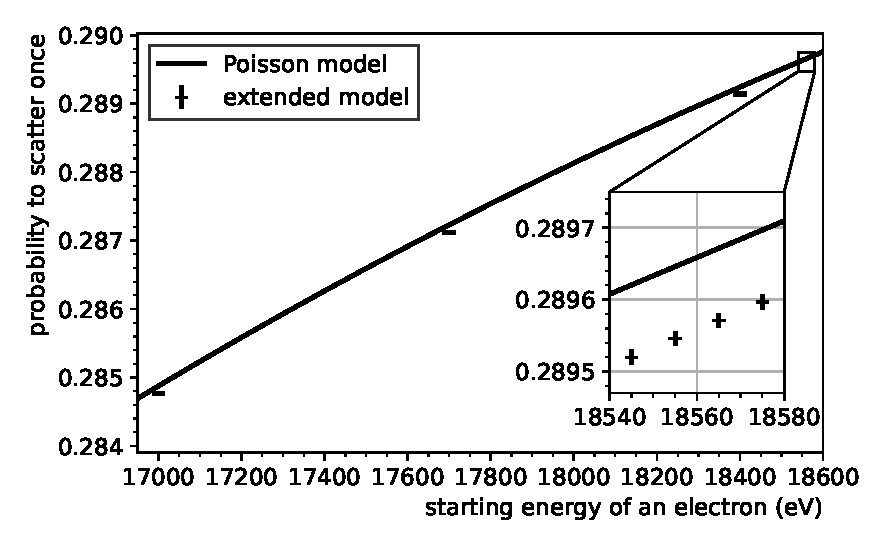
\includegraphics{chapter/energyDependentCrossSec/fig/scatProbs1PoissonAndExtended.pdf}
	\xcaption{Comparison of the Poisson and the extended model for one-fold scattering of electrons in the \glsentryshort{wgts}}{Comparison of the Poisson and the extended model for one-fold scattering of electrons in the \glsentryshort{wgts}.}{The line shows the Poisson model and the markers the extended model (see main text for a description of the models). Due to long program run times, the latter was only evaluated at a selection of energies. Furthermore, the numerical evaluation of the extended model is subject to an error of $\sim10^{-5}$ (see section~\ref{sec:eDepScatCrossSecExtendedModelNumEval}), that is depicted as uncertainty bars. The difference of the two models is $\sim10^{-4}$.}
	\label{fig:eDepScatCrossSecExtendedModelResults}
\end{figure}
For no scattering, the extended model and the Poisson model are equivalent as shown in equation~\eqref{eq:eDepScatCrossSecExtendedModelFormalismRecoveryOfPoisson}.

Figure~\ref{fig:eDepScatCrossSecExtendedModelResults} depicts the Poisson model as per equation~\eqref{eq:eDepScatCrossSecModelPoisson} and the extended model as per equation~\eqref{eq:eDepScatCrossSecExtendedModelFormalismAveragedDepScatProbs} for the probability of one-fold scattering. The difference between the two models is below $10^{-4}$.

For two-fold scattering and higher scattering multiplicities the extended model could not yet be evaluated due to the computational complexity. However an estimation based on theoretical arguments is given below.

\paragraph{Difference of the Extended and the Poisson Model for Electron Scattering}
The reasoning concerning the sign of the difference between the Poisson and the extended model is similar to the one in section~\ref{sec:eDepScatCrossSecModelPoisson} about the change of the scattering probabilities with decreasing or increasing energy: The Poisson model underestimates the total amount of scattering, because it neglects that an electron that scatters loses energy and becomes more likely to scatter again. As already shown, according to the Poisson model, electrons are expected to scatter between one and two times when traveling through the \gls{wgts} (see equation~\ref{eq:eDepScatCrossSecModelPoissonExpectedScatCount}). The extended model is more correct than the Poisson model and hence should yield an increased expected amount of scattering. Therefore, the probability for one-fold scattering should be smaller than the one given by the Poisson model (this is the case as depicted in figure~\ref{fig:eDepScatCrossSecExtendedModelResults}). For higher scattering multiplicity (which could not be calculated), the sign of the difference between the Poisson and the extended model should be the opposite. In other words, the probability of two-fold scattering as given by the Poisson model should be to low.

Also, the extended model should be a probability distribution and the sum over all scattering multiplicities should yield unity in the same manner as it does for the Poisson model (see appendix~\ref{sec:appendixEDepScatCrossSecPoissonModelProbDensityProof} for a proof that the Poisson model is a probability density). This means that for higher scattering multiplicities, the difference between the extended model and the Poisson model would have to sum up to the difference in the probability for one-fold scattering. Hence, for scattering of higher multiplicity, the absolute difference between the extended model and the Poisson model would not be able to surpass $10^{-4}$.

\paragraph{The Extended Model for Electron Scattering in Neutrino Mass Inference}
How the error of the Poisson model propagates to neutrino mass inference and whether it would introduce a significant systematic shift of the squared neutrino mass was not probed in the scope of this thesis because the current stage of the extended model is computational too demanding to be used in a fitting procedure. However, some considerations are given below:

The difference between the extended model and the Poisson model for one-fold scattering is $\sim10^{-4}$, which might be a significant scale because it is similar to the scale on which the probability for one-fold scattering changes when transitioning from an energy-independent to an energy-dependent cross section (see insets of figure~\ref{fig:eDepScatCrossSecModel}). And in the previous section~\ref{sec:eDepScatCrossSecNuMassInfThisWork}, it is shown that neglecting such an effect might lead to a systematic shift of the squared neutrino mass on the order of $\SI{e-2}{eV^2}$. Nonetheless, the difference of the extended and the Poisson model might be partly compensated by the different fit parameters such as the signal amplitude or the endpoint of the $\upbeta$ spectrum. Therefore, it was found difficult to make quantifiable assumptions.

In the following, a procedure is outlined, that might make it possible to estimate the induced systematic shift of the squared neutrino mass in a future study: One could simulate data using the Poisson model and additionally introduce an artificial negative shift on the order of $10^{-4}$ on the probability for one-fold scattering and a positive shift that is smaller than $10^{-4}$ for the probability for scattering of higher multiplicities because this should approximately resemble the extended model. The fit model can then use the Poisson model without modification. This procedure might make it possible to quantify whether there is a significant shift of the inferred squared neutrino mass caused by neglecting that electrons become more likely to scatter again if they have already scattered.

\section{Conclusion and Outlook}
\label{sec:eDepScatCrossSecConclusion}
The cross section for inelastic scattering off tritium molecules within the \gls{wgts} depends on the energy of the incident electrons. An approximated model that used the Poisson distribution was used to estimate the systematic shift on the squared neutrino mass that would be introduced if the energy dependence were neglected. The shift would be $\Delta\nuMass^2 = \SI{1.09e-2}{eV^2}$ in a \SI{30}{eV} analysis interval.

It was also shown that including the energy-dependence in neutrino mass inference via the Poisson model increases the run time of the fitting procedure by a factor of up to 140. A suggestion for an improvement of the performance via interpolation of the scattering probabilities is made in section~\ref{sec:eDepScatCrossSecModelPoissonProperties}.

The usage of the Poisson distribution underestimates the total amount of scattering, because it neglects that an electron that scatters loses energy and becomes more likely to scatter again. This does not influence the probability for no scattering. However, using the approximation of a fixed energy loss $\epsilon=\SI{12.6}{eV}$ per scattering, it could be shown that the probability for one-fold scattering would be shifted by less than $10^{-4}$. The effect on scatterings of higher multiplicities or the effect in neutrino mass inference could not be fully quantified, but an approach that might enable the quantification in the future is outlined in section~\ref{sec:eDepScatCrossSecExtendedModelDiscussion}.

The model building in this chapter was based on well argued considerations. Nonetheless, an independent cross-check is recommended. A future study might perform a Monte Carlo particle tracking simulation in order to verify the suggested models presented in this thesis.

    
    \chapter{(Theoretical Corrections to the \texorpdfstring{$\upbeta$}{Beta} Decay Spectrum)}
    \section{Motivation}
    What are theoretical corrections?
    
    \section{Application to Data}
    What is the effect on the parameters of interest? How can it be explained? 
    
    
    
    \chapter{Parameter Inference at KATRIN with KaFit}
    
    \section{The KATRIN Likelihood}
    What does parameter inference mean? What does sensitivity on the neutrino mass mean? What is the likelihood? What is a Frequentist approach? What is a Bayesian approach? 
    \section{Overview of Analysis Methods}
    What are the parameters of interest? What is run stacking? What is a uniform fit? Was the neutrino mass fixed? Which energy loss model/fsd binning/...? More general, which analysis configuration was used and why?
    
    \section{Inference Algorithms}
    \subsection{Classical Minimizer}
    What algorithm is implemented in/interfaced to KaFit? What is MINUIT and MINOS? What are the pros and cons?
    \subsection{Markov-Chain-Monte-Carlo}
    What is a Markov-Chain-Monte-Carlo?  What algorithm is implemented in/interfaced to KaFit? What are the pros and cons of the method? What are the pros and cons of the different implementations?
    
    \section{Treatment of Uncertainties}
    \subsection{Nuisance Parameters}
    What are nuisance parameters? How can they be included in an analysis? What are the difficulties? How can these difficulties be circumvented?
    \subsection{Penalized Likelihood and Priors}
    What does it mean to constrain a nuisance parameter? How can penalty terms and priors be described as constraints? How do penalty terms priors compare? How does this fit in a Frequentist and Bayesian framework?
    \subsection{Monte Carlo Propagation and Covariance Matrix Approach}
    What is the Monte Carlo Propagation and the Covariance Matrix Approach. Why are they similar? Where do they differ? What is the motivation behind using them? What are the pros and cons? What is the convergence criteria for the sampling?
    \subsection{Shift Method}
    What is the shift method? What are its limitations and when is it needed?
    
    
    
    \chapter{(Energy Loss Normalization on First Tritium)}
    
    
    
    \chapter{Studies using the Preliminary KATRIN Energy Loss Model}
    \section{The Preliminary KATRIN Energy Loss Model}
     Which systematic effects were considered? What are the quantified uncertainties on them and where do these numbers come from? Why this selection?
    \section{Neutrino Mass Sensitivity}
    \subsection{Motivation}
    Why combining systematics? What was possible in the scope of this thesis? What does this thesis try to show?
    \subsection{Methodology}
    What is the sensitivity on the parameters of interest? What is the z score and shrinkage for all parameters?
    \subsection{Model Configuration}
    Which model configuration (MTD, Slicing, Eloss-Model, FSD Binning, ...) was chosen and why?
    \subsection{Results}

    \section{Application to Data}
    
    \chapter{Conclusions}

    \Appendix
    \chapter*{\appendixname} \addcontentsline{toc}{chapter}{\appendixname}
    \section{Energy-Dependent Model of the Probability for Electron Scattering within the \gls{wgts}}
\label{sec:appendixEDepScatCrossSecExtendedModel}
Section~\ref{sec:eDepScatCrossSecModel} introduces a model for the probability of electron scattering within the \gls{wgts} using the Poisson distribution. As explained, depending on the required accuracy, the conditions for using a Poisson distribution might be violated. Section~\ref{sec:appendixEDepScatCrossSecExtendedModelFormalism} introduces a model beyond the description via a Poisson distribution. Its evaluation was done numerically which demanded a trade-off between accuracy and run time. The latter is assessed in section~\ref{sec:appendixEDepScatCrossSecExtendedModelNumEval}.
\subsection{Modeling}
\label{sec:appendixEDepScatCrossSecExtendedModelFormalism}
In the following, a model for for the probability of electron scattering within the \gls{wgts} that depends on the electrons energy is derived. The difficulty lies in the fact, that an electron that scatters looses energy and hence its probability to scatter a second time is different from the first time. The presented model is inspired by a model given in~\cite{Groh2015}, that treats a similar effect for a change of an electron's pitch angles due to scattering. 

The aim is to derive an expression $\bar{P}^{\star}_l(\Esource)$ that denotes the probability of $l$-fold scattering for a $\upbeta$ electron with a starting energy $\Esource$ averaged over all starting positions and pitch angles assuming a fixed energy loss $\epsilon$ per scattering.

The expected amount of scatterings for a $\upbeta$ electron when traveling  through the whole \gls{wgts} volume of length $d$ filled with a gas of constant density $\rho$ is (see equation~\ref{eq:intSpecModelExpectedScatteringCount})
\begin{equation}
    \mu(E,\thetaSource) =
    \frac{\sigma(E)\rho d}{\cos\thetaSource},
\end{equation}
where $E$ denotes the electron's kinetic energy; $\thetaSource$ the starting pitch angle; and $\sigma(E)$ the energy dependent scattering cross section.

In the developed model, the volume of the \gls{wgts} is divided into $N$ slices of equal width $w=L/N$. $N$ is chosen sufficiently large that the probability for a $\upbeta$ electron to scatter twice within one slice is essentially zero. Then, for large $N$ the probability to scatter within one slice is $\mu(E,\thetaSource)/N$. The probability not to scatter within $n \leq N$ slices is
\begin{equation}
    p_0(E,\thetaSource,n) =
    \left(
        1-\frac{\mu(E,\thetaSource)}{N}
    \right)^n
    \fullstop
\end{equation}
Using the well known limit for the Euler constant, one obtains for $n=N$ and $N\rightarrow\infty$ that $p_0$ is a Poisson distribution with expectation $\mu$ evaluated at 0 
\begin{align}
    \lim_{N\rightarrow\infty} 
    p_0(E,\thetaSource,N) =
    \lim_{N\rightarrow\infty} 
    \left(
        1-\frac{\mu(E,\thetaSource)}{N}
    \right)^N =
    \mathrm{e}^{-\mu(E,\thetaSource)}
    \fullstop
\end{align}
In other words, for no scattering, the Poisson model for the scattering probabilities as described in section~\ref{sec:eDepScatCrossSecModel} is recovered.

Assuming a constant energy loss per scattering of $\epsilon$ the probability to scatter $l$ times within $n<N$ slices can be expressed recursively
\begin{equation}
	\label{eq:appendixEDepScatCrossSecExtendedModelFormalismCore}
    p_l(E,\thetaSource,n) =
    \underbrace{
        \sum_{k=l}^{n}
    }_{(4)}
    \underbrace{
        p_{l-1}(E,\thetaSource,k-1)
        \vphantom{\sum_{k=l}^{n}}
    }_{(1)}
    \underbrace{
    \left(
        1-p_0(E-(l-1)\epsilon,\thetaSource,1)
    \right)
    \vphantom{\sum_{k=l}^{n}}
    }_{(2)}
    \underbrace{
        p_0(E-l\epsilon,\thetaSource,n-k)
        \vphantom{\sum_{k=l}^{n}}
    }_{(3)}
    \fullstop
\end{equation}
The idea behind this expression is the following: One imagines an electron with an energy $E$ that travels through $n$ \gls{wgts} slices, scatters $l$ times in total and once in the $k$th slice. Hence, it must have scattered $l-1$ times in the $k-1$ slices and must not scatter in the $n-k$ slices to follow. In that regard, the above terms have the following meaning:
\begin{enumerate}[(1)]
    \item Probability to scatter $l-1$ times within $k-1$ slices with a kinetic energy of $E$.
    \item Probability to scatter once within the $k$th slice with a kinetic energy of $E-(l-1)\epsilon$.
    \item Probability not to scatter within the remaining $N-k$ slices.
    \item Sum over all slices $k$ where the electron could scatter the last time. The sum starts at $l$ because the probability to scatter $l-1$ times within less than $k=l-1$ slices (term (1)) is 0 because of the made assumption, that in the limit of large amount of slices $N$ an electron does not scatter twice within one very narrow slice.
\end{enumerate}
The probability to scatter $l$ times can be averaged over all starting positions
\begin{equation}
    \label{eq:appendixEDepScatCrossSecExtendedModelFormalismZAverage}
    \bar{p}_l(E,\thetaSource) = 
    \frac{1}{N}
    \sum_{\nSource=1}^{N} p_l(E,\thetaSource,\nSource) \approx
    \frac{1}{d}
    \int_{0}^{d}
        p_l(E,\thetaSource,
            \left\lceil N \frac{\zSource}{d}\right\rceil
        )
    \d \zSource
    \fullstop
\end{equation}
Here, the averaging sum is approximated by an integral as this helps cutting down on run time in a numerical evaluation. This is due to the fact, that in a numerical evaluation a large number $N$ ($\sim10^5$) of slices has to be chosen and the sum would have many terms. However, a numerical integration can achieve an accurate result with a smaller set of supporting points (see subsequent section~\ref{sec:appendixEDepScatCrossSecExtendedModelNumEval}). 

In the formal expression, the limit $N\rightarrow\infty$ can be applied
\begin{equation}
  P^{\star}_l(\Esource,\thetaSource) = 
    \lim_{N\rightarrow\infty} \bar{p}_l(\Esource,\thetaSource)
    \label{eq:appendixEDepScatCrossSecExtendedModelFormalismPitchAngleDepScatProbs}
\end{equation}
$P^{\star}_l(\Esource,\thetaSource)$ denotes the probability for a $\upbeta$ electron to scatter $l$ times when traveling through the whole \gls{wgts} with a starting energy $\Esource$ and pitch angle $\thetaSource$ averaged over all starting positions. Finally, this expression can be averaged over all starting pitch angles in order to obtain the energy dependent scattering probabilities
\begin{equation}
    \bar{P}^{\star}_l(\Esource) = 
    \frac{1}{1-\cos\thetaMax}
    \int_0^{\thetaMax}
    	\sin \thetaSource
        P^{\star}_l(\Esource,\thetaSource) 
        \d \thetaSource
    \fullstop
    \label{eq:appendixEDepScatCrossSecExtendedModelFormalismAveragedDepScatProbs}
\end{equation}
$\bar{P}^{\star}_l(\Esource)$ denotes the probability of $l$-fold scattering for a $\upbeta$ electron with a starting energy $\Esource$ averaged over all starting positions and pitch angles assuming a fixed energy loss $\epsilon$ per scattering. To derive such an expression was the aim of this section. 

\subsection{Numerical Evaluation and Cross-Check}
\label{sec:appendixEDepScatCrossSecExtendedModelNumEval}
\begin{figure}[t]
    \centering
    \includegraphics{chapter/energyDependentCrossSec/appendix/fig/scatProb1_numericalAccuracy.pdf}
    \xcaption{Numerical accuracy of the extended model for the probability of electron scattering within the \gls{wgts}}{Numerical accuracy of the extended model for the probability of electron scattering within the \gls{wgts}.}{The extended model is given by \eqref{eq:appendixEDepScatCrossSecExtendedModelFormalismAveragedDepScatProbs}. The Poisson model is given by equation~\eqref{eq:eDepScatCrossSecModelPoisson}. For both models the energy of the incident electrons was taken as $\SI{18764.4}{eV}$ because for this energy, the Poisson model yields the values already given in table~\ref{tab:eDepScatCrossSecModelScatProbs}. The left column shows the dependence on the number $N$ of slices of the \gls{wgts}. The right column shows the dependence on the order of Gaussian quadrature that was used to evaluate the two integrals in the extended model. The Poisson model is independent of these features and can be evaluated exactly. For the left column the order of Gaussian quadrature was fixed to 5. For the right column the number of slices was fixed to $5\times10^{5}$. The upper row shows the numerical evaluation of the extended model for no energy loss per scattering (markers). Its exact solution is given by the Poisson model (line). The lower row shows the model for an energy loss of \SI{12.6}{eV} per scattering. These results make it plausible to assume a one-sided numerical inaccuracy on the $10^{-5}$ level for $N=5\times10^5$ and using Gaussian quadrature of order 5 for the numerical evaluation of the extended model.}
    \label{fig:appendixEDepScatCrossSecExtendedModelNumEval}
\end{figure}
The energy-dependent probability $\bar{P}^{\star}_l$ for electrons to scatter $l$-fold (extended model) in equation~\eqref{eq:appendixEDepScatCrossSecExtendedModelFormalismAveragedDepScatProbs} was evaluated numerically. Taking the limit~$N\rightarrow\infty$ in equation~\eqref{eq:appendixEDepScatCrossSecExtendedModelFormalismPitchAngleDepScatProbs} was replaced by choosing a large $N$. The averaging integral over the starting positions in equation~\eqref{eq:appendixEDepScatCrossSecExtendedModelFormalismZAverage} and starting pitch angles in equation~\eqref{eq:appendixEDepScatCrossSecExtendedModelFormalismAveragedDepScatProbs} was computed using Gaussian quadrature. The extended model was introduced because the preconditions to model the scattering probabilities via a Poisson distribution (Poisson model) do not hold. Hence, the numerical evaluation of the extended model must be sufficiently accurate to show the difference to the Poisson model. How accurate this is, can not be known beforehand and was found out by trial and error. Both, $N$ and the order of Gaussian quadrature, should be chosen as low as possible to cut down on run time, but sufficiently high for the required accuracy. 

Also, a benchmark had to be found, to determine the accuracy of the numerical evaluation. The following idea was used: For an energy loss of $\epsilon=\SI{0}{eV}$ per scattering, the extended model must recover the Poisson model exactly. This can be used to estimate the numerical accuracy in dependence of the number $N$ of slices and order of Gaussian quadrature. The estimated accuracy for $\epsilon=\SI{0}{eV}$ was then assumed for $\epsilon>\SI{0}{eV}$. A further cross-check is to look at the convergence of the numerical evaluation with increasing $N$ and an increasing order of the Gaussian quadrature.

The averaged probability for 1-fold scattering $\bar{P}^{\star}_1$ of the extended model, was evaluated for $\epsilon=\SI{0}{eV}$. The result in dependence of $N$ and the order of the Gaussian quadrature is shown in the top row of figure~\ref{fig:appendixEDepScatCrossSecExtendedModelNumEval}. It should recover th Poisson model. For $N=5\times10^5$ and using Gaussian quadrature of order 5, the Poisson model and the extended model differ less than $3\times10^{-6}$. Furthermore, the numerical calculation converges from below, which may be interpreted as a one-sided numerical inaccuracy. The calculations for $\epsilon=\SI{12.6}{eV}$ are shown in the lower row of figure~\ref{fig:appendixEDepScatCrossSecExtendedModelNumEval}. They also show convergence on the $10^{-5}$ level. Conclusively, the results make it plausible to assume a one-sided numerical inaccuracy on the $10^{-5}$ level for $N=10^5$ and using Gaussian quadrature of order 5 for the integrals.

The corresponding run time to compute $\bar{P}^{\star}_1$ is in $\mathcal{O}(N)$ as it requires a sum over all $N$ slices in equation~\ref{eq:appendixEDepScatCrossSecExtendedModelFormalismCore}. The extended model is defined recursively and therefore, the run time for $l$-fold scattering is in $\mathcal{O}(N^l)$. Hence, computing the probability for two-fold scattering would take $5\times10^5$ times as long as for one-fold scattering for the same $10^{-5}$ accuracy. This was not yet found to be feasible.
\FloatBarrier
    
    
    \section{First Tritium Data}
    What is First Tritium? Which data was selected?
    
    \glsaddall
    \printglossary[type=\acronymtype]
    \TheBibliography
    \printbibliography
    % \nocite{*} or maybe \nocite{Kon64,And59} for specific entries
    %\nocite{*}
    %\bibliographystyle{babalpha}
\end{document}
